\chapter{Modelagem Matemática}
\pagestyle{simple}
\label{cap:modelagem}

Visando permitir o uso do poder computacional na busca de uma solução para o problema apresentado no capítulo \ref{cap:problema}, necessita-se modelar o problema de forma matemática.

Dessa forma foi optado o uso da teoria dos grafos como estrutura matemática visando modelar o problema.

\section{Conceitos Gerais em Teorias dos Grafos}

Um grafo simples $G(V,E)$ é definido por \citeonline{szwarcifter86} como sendo uma estrutura matemática composta por um conjunto finito não vazio de vértices $V$ e um conjunto $E$ de pares, não ordenados, de diferentes vértices denominados arestas.

%% inserir imagem
%%  --- Grafo
\begin{figure}[H]
     \centering
     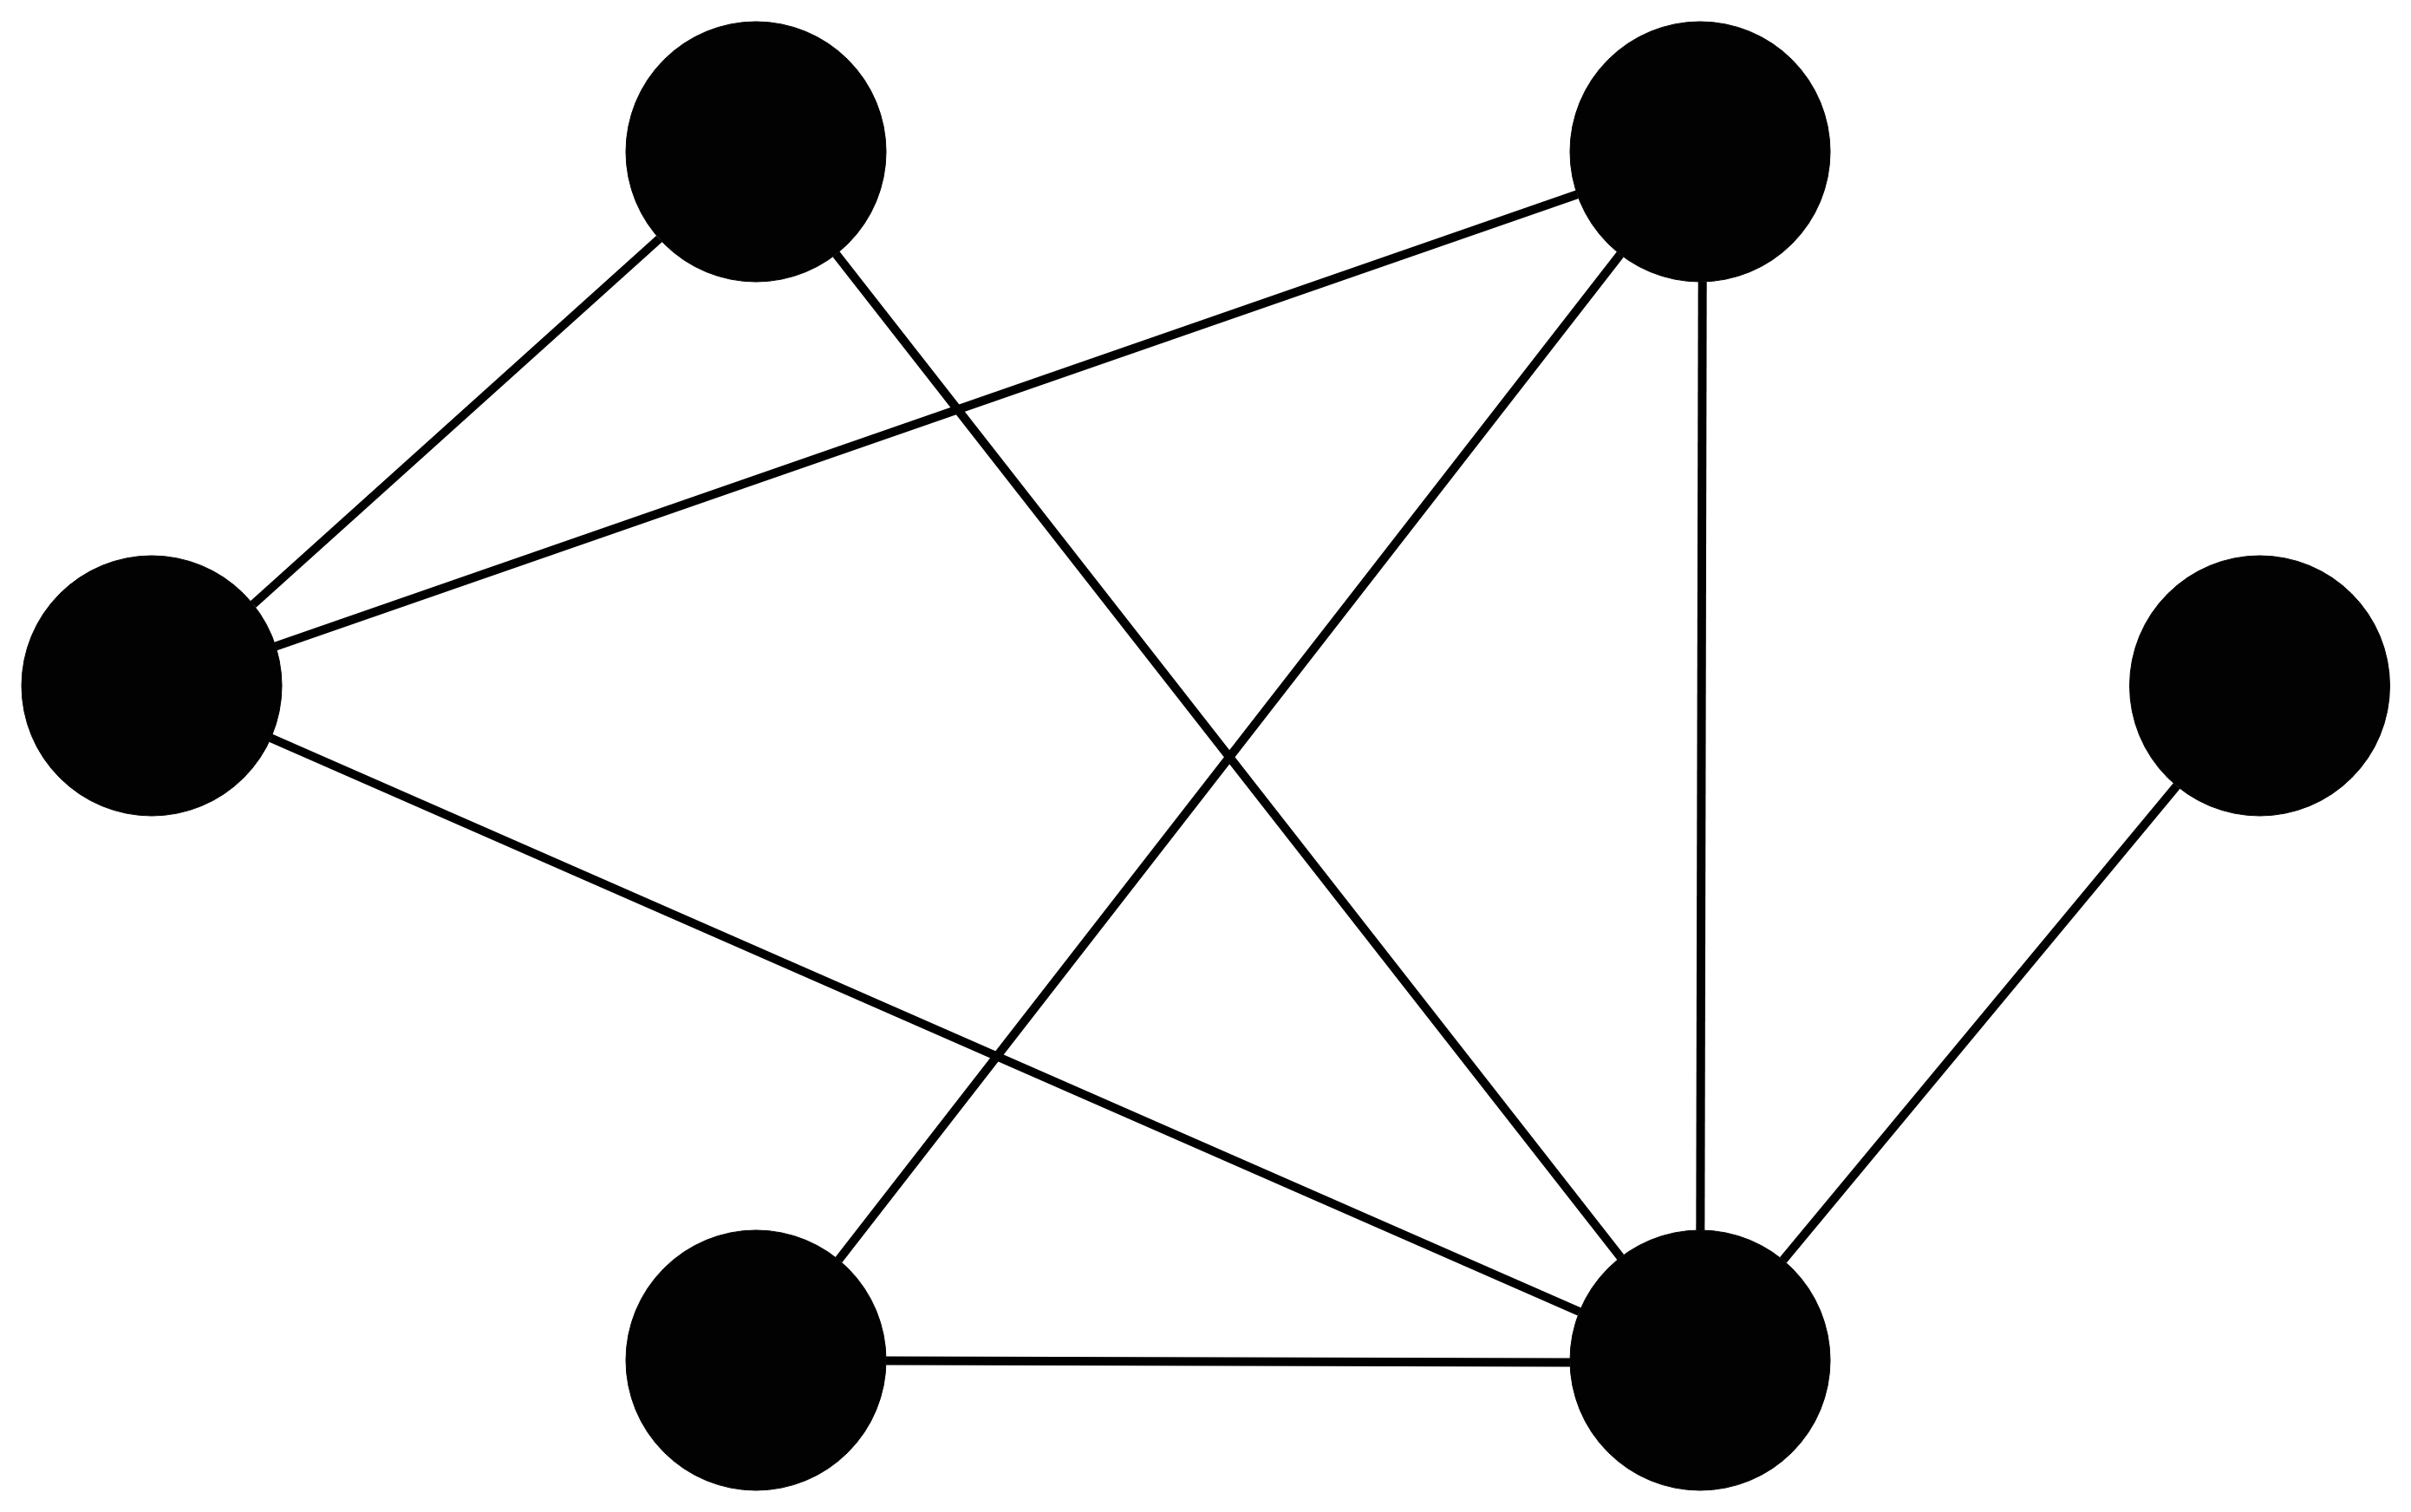
\includegraphics[width=0.6\textwidth]{TCC/imagens/grafos/grafo.png}
     \caption{Representação geométrica de um Grafo}
     \label{Representação geométrica de um grafo}
\end{figure}


Um grafo é comumente representado graficamente conforme a figura \ref{Representação geométrica de um grafo}, onde os vértices são representados por círculos e as arestas por linhas que interligam dois vértices.

Elementos componentes de um grafos conforme definidos por \citeonline{szwarcfiter18} e \citeonline{pinto18} a seguir.


\begin{definition} 
 \textbf{Vértice}: um vértice é denotado por $V(G)$ é representado graficamente através de um ponto, a quantidade dos vértices de um grafo é expressa por $|V|$, onde um grafo com $|V| = 1$ é classificado como um grafo trivial.
 \end{definition}

\begin{definition} 
\textbf{Aresta}: uma aresta $e \in E(G)$ é denotada por um par de vértices $e = (v,w)$. Dessa forma os vértices $v$ e $w$ estão conectados as extremidades da aresta e, dessa forma são denominados adjacentes. Já uma aresta é denominada incidente aos vértices em seus extremos $v$ e $w$.
\end{definition}

\begin{definition} 
\textbf{Grau de um vértice}: o grau de um vértice $v \in V(G)$, é denotado por grau($v$), sendo esse o número de vértices adjacentes a $v$.
\end{definition}

\begin{definition} 
\textbf{Multigrafo}: denotado por $H(V,E)$, é um grafo que admite diferentes arestas incidentes a um mesmo par de vértices $(v,w)$ ou laços, sendo arestas que são incidentes a um único vértice ($v$,$v$).
\end{definition}

\begin{definition} 
\textbf{Grafos Direcionados}: em um grafo direcionado (digrafo) $D(V,E)$ é um conjunto finito não vazio $V(G)$ (os vértices), e um conjunto $E(G)$ (as arestas) de pares ordenados de vértices distintos. Portanto, também que ($v$,$w$) possui uma única direção de $v$ para $w$.
\end{definition}

\begin{definition} 
\textbf{Grafo Ponderado em Arestas}: um grafo é classificado como ponderado quando é atribuído um valor (peso) $p$ as arestas, sendo esse $p(v,w)$ ou $p(e)$.
\end{definition}

\begin{definition} 
\textbf{Rótulo}: um rótulo consiste na atribuição de um valor (numérico ou alfabético) que simbolize ou represente um elemento do grafo de modo a facilitar a identificação de um vértice ou aresta específica em uma representação.
\end{definition}

% Área da matemática muito estudada na computação.
A Teoria dos Grafos é uma área amplamente estudada tanto na matemática quanto na computação. Muitos problemas do mundo podem ser descritos como problemas de grafos, dessa forma, ao se propor uma solução para o modelo de grafos também de obtém a solução para o problema real.

Muitos problemas e soluções já foram propostos com o passar dos anos, isso possibilita que a teoria dos grafos tenha modelos que se adéquem a muitas descrições, e algoritmos (sequência de instruções para se fazer uma operação no computador) eficientes para resolvê-los.

\section{Exemplos de problemas modelados com Grafos}

Atualmente muitos serviços tecnológicos utilizam das estruturas de grafos para resolverem problemas do dia-a-dia das pessoas. Esses serviços podem ser aplicativos para \textit{smartphones}, sistemas \textit{web} ou até mesmo sistemas \textit{desktop}.

Dentre os aplicativos que utilizam de modelos em grafos para resolver seus problemas, destacam-se os seguintes exemplos:


\subsection{\textit{Facebook} e \textit{Twitter}}
    
As mídias sociais que se popularizaram desde a criação da “internet”, muitas podem ter suas aplicações modeladas com uso de grafos, e não apenas isso, mas algumas dessas mídias são criadas de forma a obter benefícios dessas estruturas.

Dois exemplos podem ser destacados pela forma diferente de se utilizar a estrutura dos grafos, o \textbf{\textit{Facebook}} e o \textbf{\textit{Twitter}}. 
    
    O \textit{Facebook} pode ter as relações de amizade representadas como um grafo simples, onde duas pessoas que sejam amigos na plataforma representariam uma relação. Nesse caso cada usuário será representado por um vértice $v \in V$, e usaremos uma aresta ($v$, $w$) para representar relações de amizade entre dois usuários. Como apresentado na figura \ref{grafo-facebook}.
    
    \begin{figure}[H]
         \centering
         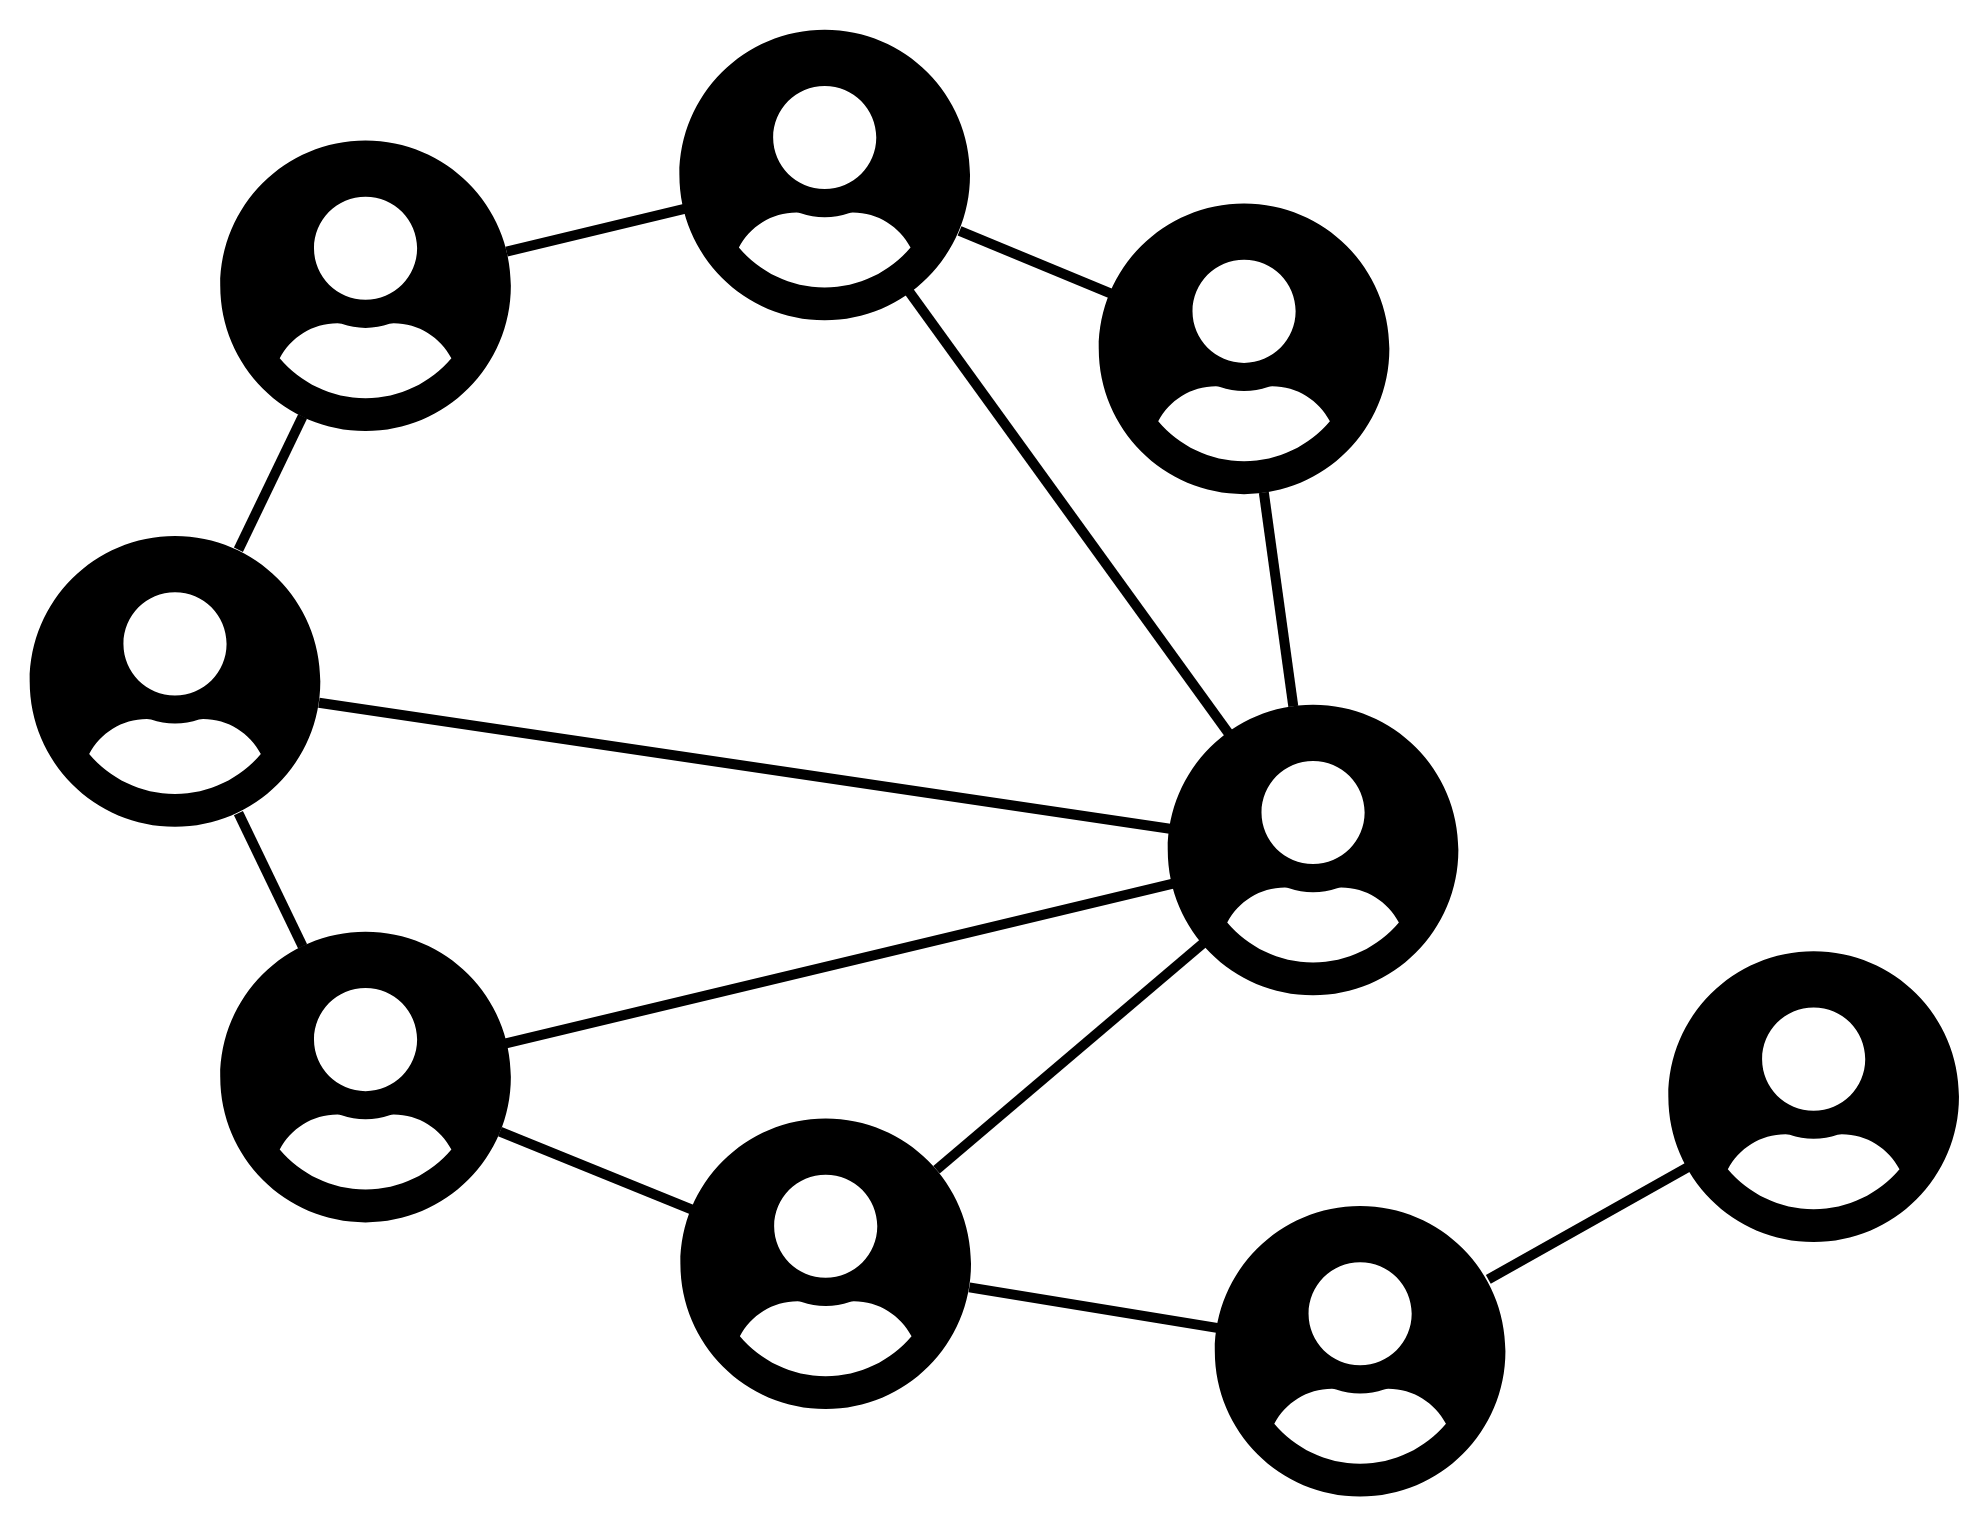
\includegraphics[width=0.6\textwidth]{TCC/imagens/grafos/grafo-facebook.png}
         \caption{Representação de uma rede de amigos do \textit{Facebook} como um Grafo}
         \label{grafo-facebook}
    \end{figure}

Diferente do caso do \textit{Facebook}, onde para termos uma relação de amizade precisamos que os dois usuários sejam amigos entre si, o \textit{Twitter} apresenta o conceito de seguir outros usuários, e não necessariamente ser seguido por eles.

Dessa forma, a representação dessas relações seriam expressas melhor por um multigrafo direcionado, onde os usuários são representados pelos vértices $v$, e uma aresta ($v$, $w$) representará aqueles que ele segue, sendo essas arestas com sentido, com a origem no usuário que segue $v$ e o destino no usuário que é seguido $w$. Dessa forma podemos observar essas diferenças na figura \ref{grafo-twitter}.
    
    \begin{figure}[H]
         \centering
         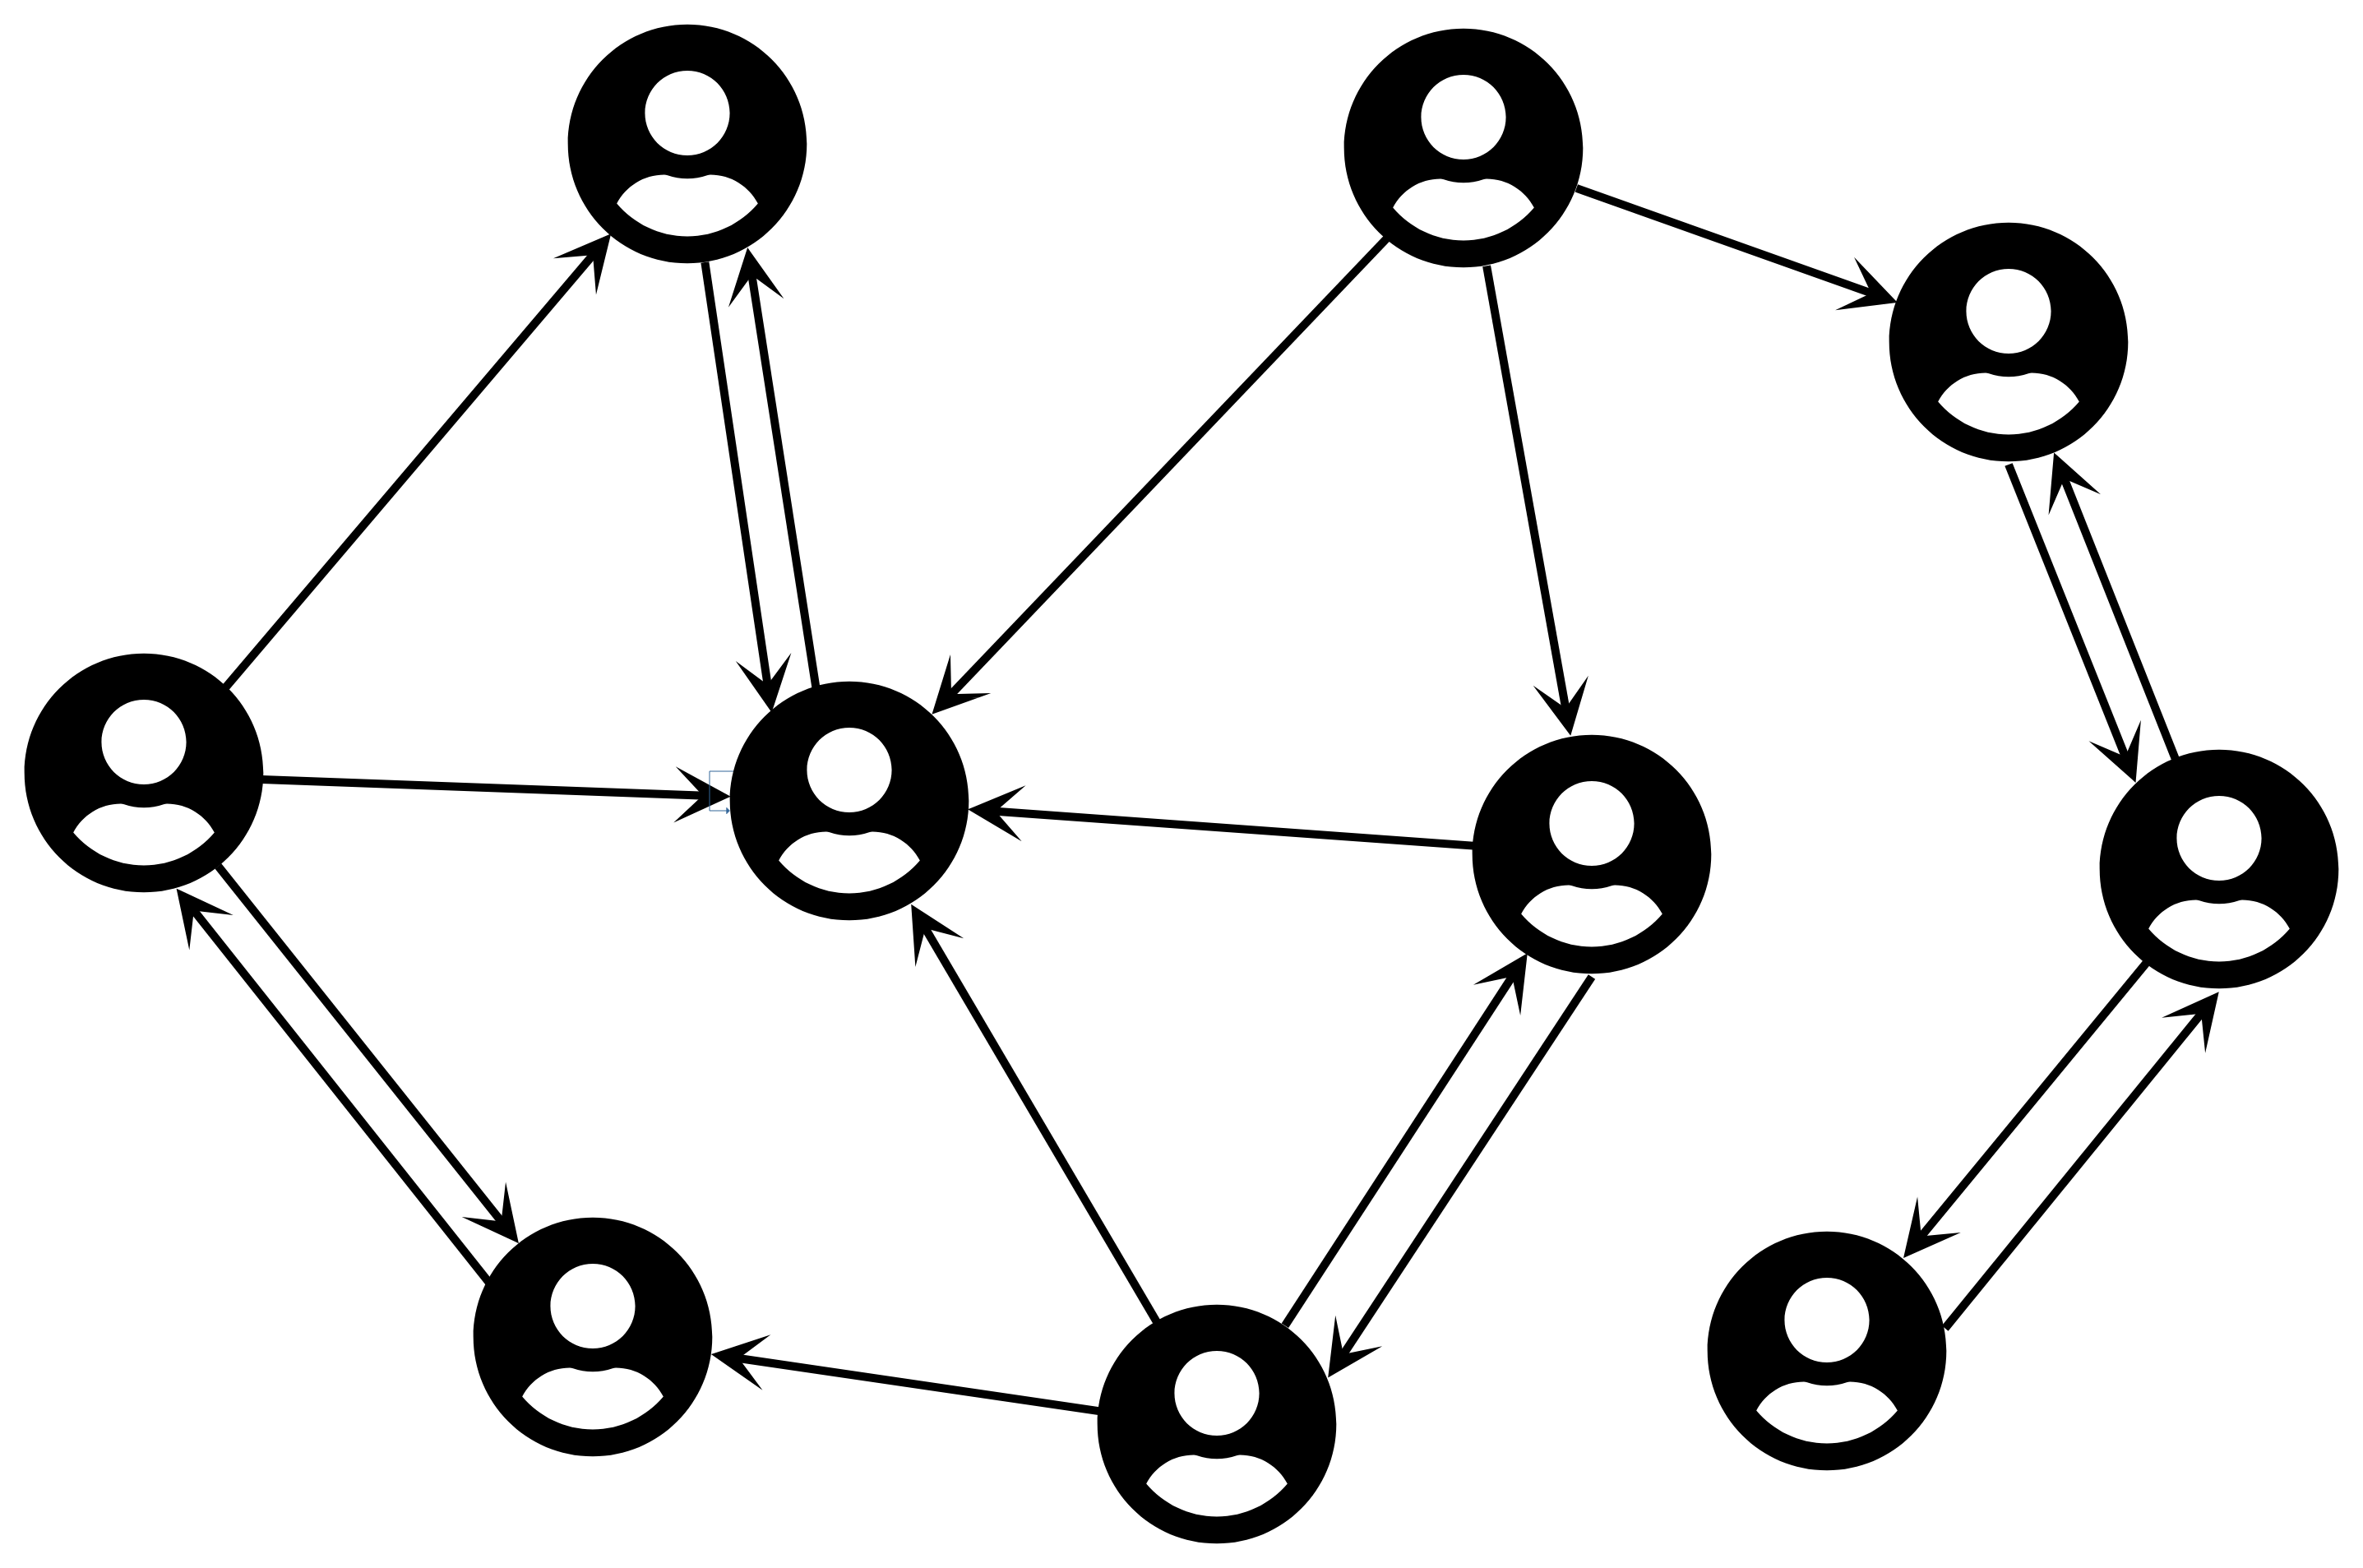
\includegraphics[width=0.6\textwidth]{TCC/imagens/grafos/grafo-twitter.png}
         \caption{Representação de rede de seguidores do \textit{Twitter} como um Grafo}
         \label{grafo-twitter}
    \end{figure}
    
    
    
    \subsection{\textit{Google Maps} e \textit{Waze}}
    
Aplicativos de geolocalização atuais podem utilizar grafos para determinar melhores rotas, podemos considerar como vértices os locais (ou pontos de referência) no qual o usuário deverá passar, e as arestas como o percurso que interligará esses dois pontos.

De acordo com a necessidade, o grafo pode ganhar informações adicionais, como pesos atribuídos as arestas, simbolizando a distância entre dois pontos, ou a velocidade média de outros veículos na travessia entre os dois pontos, esses fatores serão considerados para se propor uma rota, seja a que cruze o menor número de pontos, a que percorra a menor distância total, ou que obtenha a maior velocidade média de modo a percorrer em menor tempo a rota.
    
    \begin{figure}[H]
         \centering
         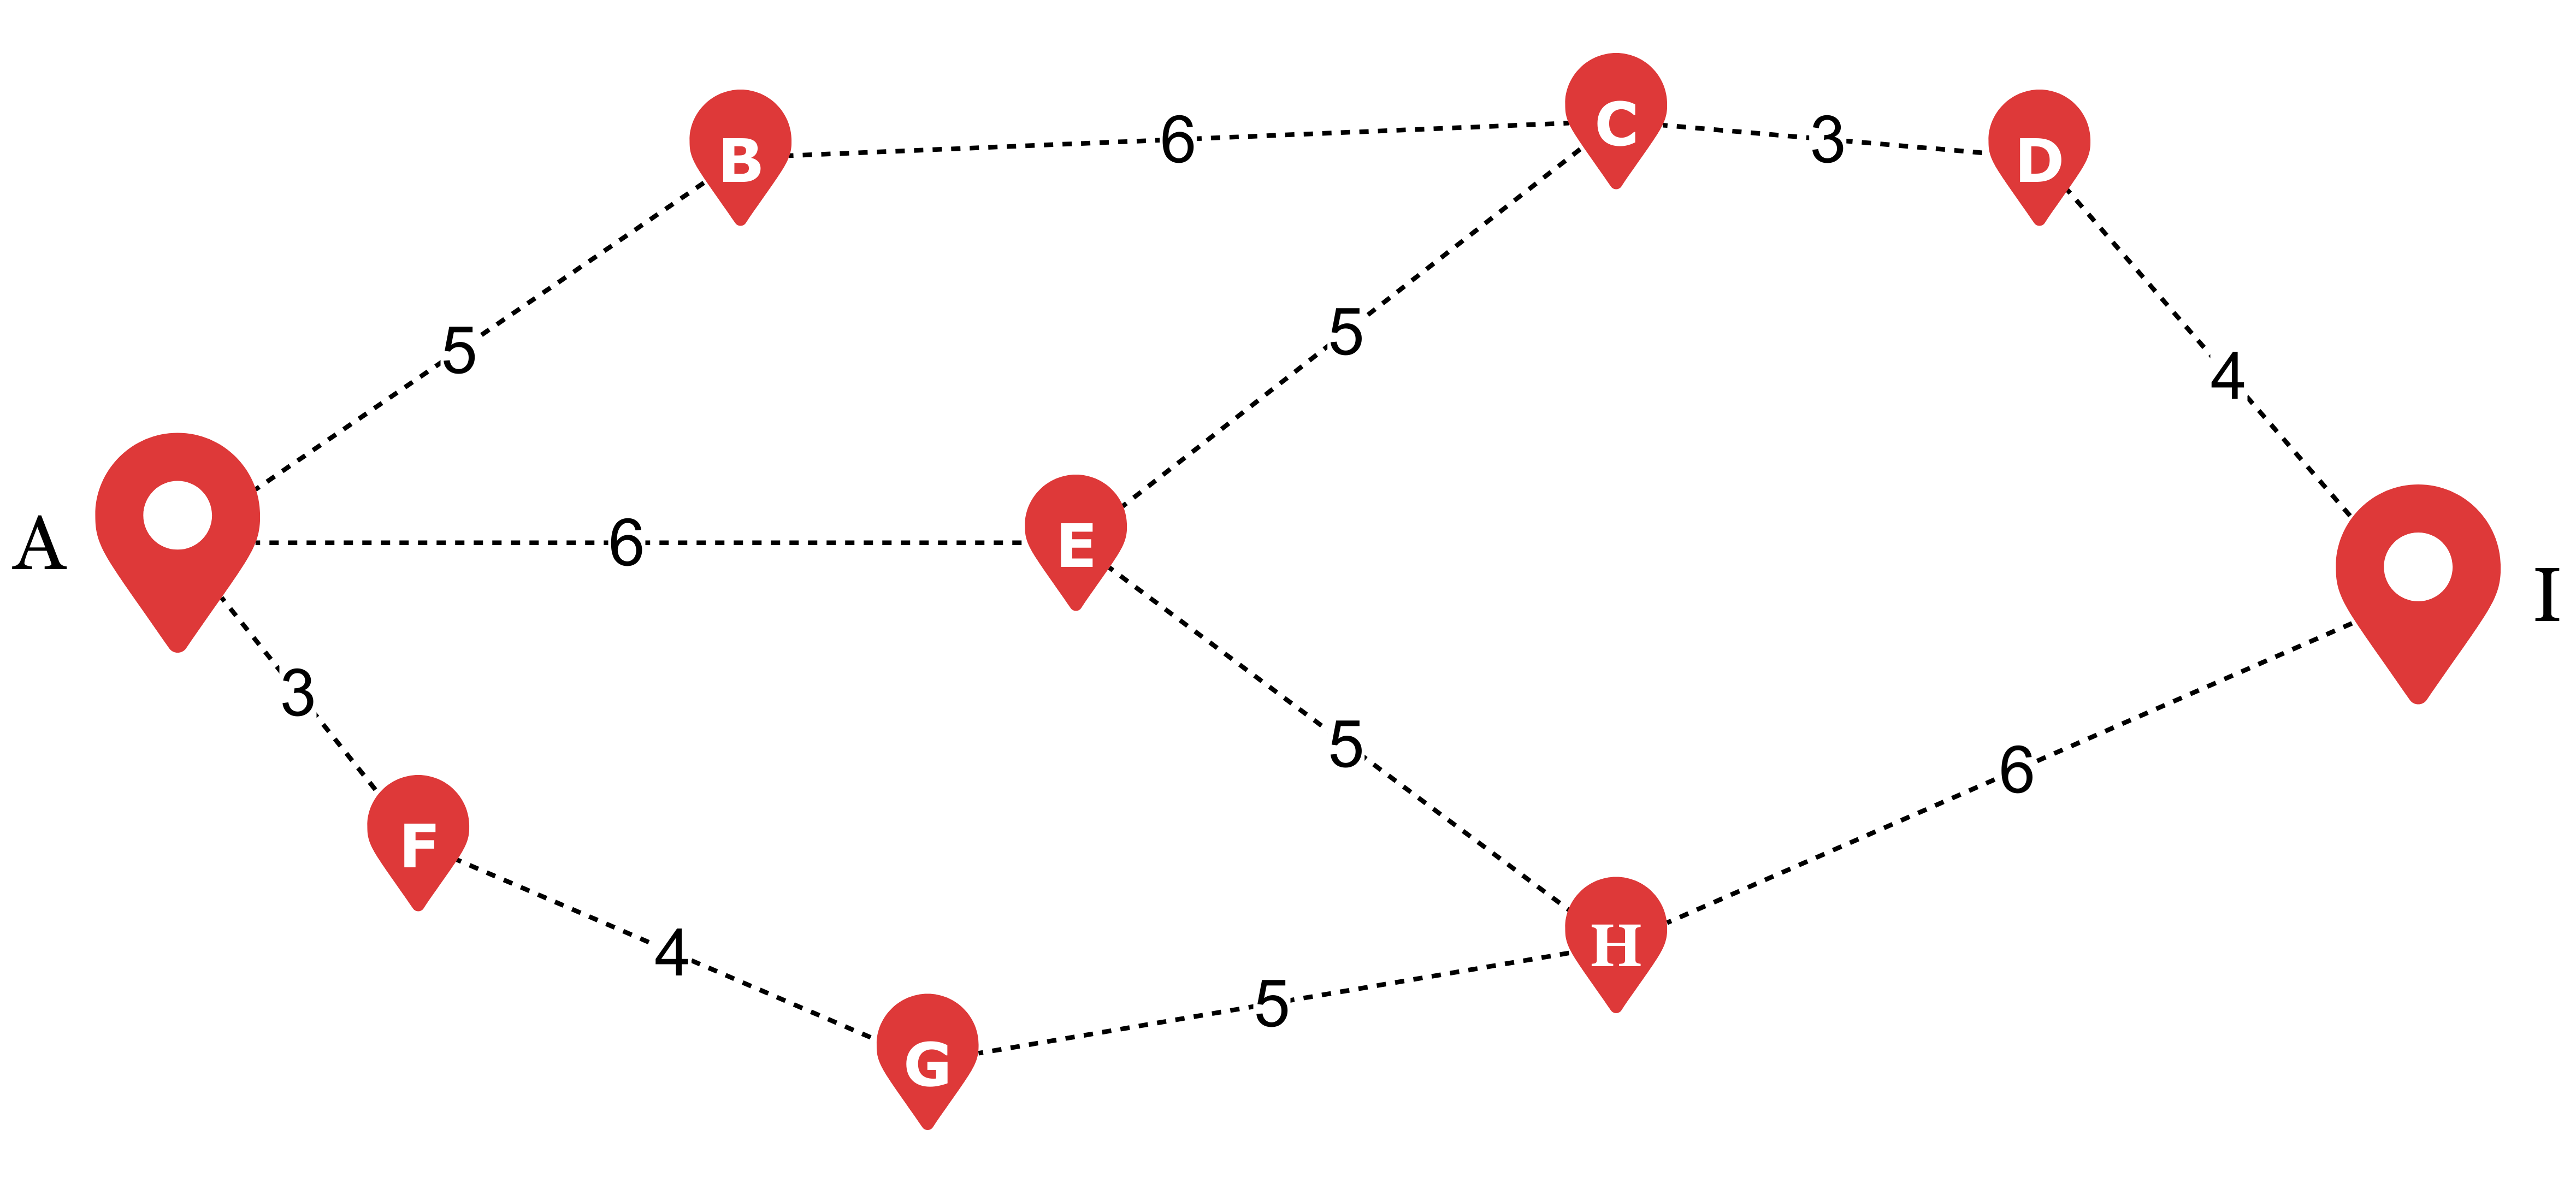
\includegraphics[width=0.6\textwidth]{TCC/imagens/grafos/grafo-maps.png}
         \caption{Representação de mapa de rotas como um Grafo}
         \label{Representação de gráfica de um grafo}
    \end{figure}
 
    
    

    
    




%%
 %%   \section{Definição do Problema Matemático}
 %%   \label{sec:def_prob}
    
 %%    Usando a notação de \cite{goldbarg_05} denotamos como: "Sendo o conjunto $M = \{1, 2, ..., m\}$ e um conjunto $f = \{ M_{1}, M_{2}, ..., M_{n}\}$ uma família de subconjuntos de $M$, onde $ M_j  \subseteq M $ e $ j \in J = \{1, 2, ..., n\} $”.
 %%    Observamos que $M_j \cap M_i \geq 0$, tendo $i \in J$ e $i \neq j$. 
    
%%    Buscando-se particionar os elementos de $f$ em $k$ partes, temos que $P = \{p_1, p_2, ..., p_k\}$ e $P \subseteq f$. 
    
 %%   Busca-se então particionar os elementos de $f$. Sendo $P_{p}$ uma partição $p$ de $\Omega$, com $p \in \{1,...,k\}$. Denotamos $S_p = |\bigcap\limits_{}^{} A'|,\; \forall A ”\in P_{p}$, ou seja, $S_{p}$ é o número de elementos existentes nas interseções entre os conjuntos que pertencem a partição $p$. Definimos também, $S$ como a soma de todos os $S_{p}$ de uma solução, ou: $\sum\limits_{i = 0}^{k}S_{p}$. 
    
  %%  Tendo $ S ”= | \bigcap\limits_{i = 0}^{n} A_{i} |$, e $Q$ um índice de qualidade de uma solução qualquer. Definimos que:
    
 %%   \begin{equation} \label{eq:qualidade}
 %%    Q = \frac{S \times 100}{S'}
  %%  \end{equation}
    
  %%  O objetivo nesse cenário se encontra em obter uma solução que possua o menor valor possível para $Q$, onde 0 seria a solução ótima para o problema, e 100 a pior solução possível. 
    
%%    Uma solução é definida aqui como: um $k$-particionamento qualquer de $\Omega$.
    
    
    % (imagem ilustrativa com N conjuntos de M elementos cada, sendo separada em K partições)
    
    %\subsection{Classificação do Problema}
    
  %%  Ao realizar uma analogia do o problema de \textit{Alocação de Turmas em Horários de Prova}, enunciado em \ref{subsec:desc_prob}, com as definições aqui apresentadas, observamos que: 
    
  %%  \begin{itemize}
  %%  \item[(a)] $\Omega$ corresponderá à uma instituição;
 %%   \item[(b)] um elemento $A_{i} \in f$ será correspondente a uma turma qualquer, onde $i$ representa uma turma específica;
 %%   \item[(c)] uma partição $P$ equivalerá à um horário de prova;
 %%   \item[(d)] e $S$ será o número de provas de segunda chamada necessárias, tendo $S_{p}$ como o número de conflitos obtidos em um horário $p$.  
%%    \end{itemize}
    
    

\section{Grafo de Interseção de Turmas}


\citeonline{pinto18} define um grafo de interseção, quando seja possível esse grafo $G(V, E)$ representar as relações entre elementos de um conjunto através das relações entre seus vértices $v \in V$.

Para modelarmos nosso problema original na forma de um grafo, será necessário ainda ressaltar algumas das características pertencentes ao problema estudado.

Observando uma instituição universitária, suas turmas têm caráter diferente do contexto escolar (ensino fundamental e ensino médio), em uma universidade as turmas são equivalentes uma disciplina que pode ser ofertada a um grupo de alunos, onde esses podem se inscrever nela ou não, de acordo com as normas estabelecidas pela instituição e vontade do aluno.

Um aluno, dessa forma, irá se inscrever em uma série de turmas todo semestre letivo. Cada turma terá ao início de cada semestre uma lista de alunos inscritos.

Para modelar essas turmas em um grafo de interseções, iremos primeiramente observar as listas de alunos inscritos nas turmas da instituição, como no exemplo mostrado a seguir na tabela \ref{tabela-lista-turmas}.

\begin{table}[H]
    \centering
    \vspace{0.5cm}
    \renewcommand\arraystretch{1.5}
    \begin{tabular}{c|c|c|c}
     
        \textbf{Turma A} & \textbf{Turma B} & \textbf{Turma C} & \textbf{Turma D} \\ % Note a separação de col. e a quebra de linhas
        \hline                               % para uma linha horizontal
        001   &   003  &   001   &   020  \\
        002   &   006  &   003   &   021  \\
        003   &   009  &   006   &   022  \\
        004   &   011  &   009   &   023  \\ 
        005   &   012  &   011   &   024  \\ 
        006   &   013  &   012   &   025  \\ 
        007   &   014  &   013   &   026  \\ 
        008   &   015  &   018   &   027  \\ 
        009   &   016  &   019   &   028  \\ 
        010   &   017  &   020   &   029     % não é preciso quebrar a última linha
        \\
        \hline
    \end{tabular}
    \caption{Lista de turmas e a matrícula seus respectivos alunos}
    \label{tabela-lista-turmas}
\end{table}

Observamos que essa instituição possui quatro turmas, com dez alunos em cada turma.

As turmas nesse exemplo são: “turma A', “turma B', “turma C ”e “turma D'. Nesse cenário iremos atribuir um vértice para cada turma, sendo o rótulo do vértice a letra que representa a respectiva turma (A, B, C e D).

Ao realizar esse processo teremos como resultado o grafo da figura \ref{grafo-turmas1}, com quatro vértices, um para cada turma.

\begin{figure}[H]
     \centering
     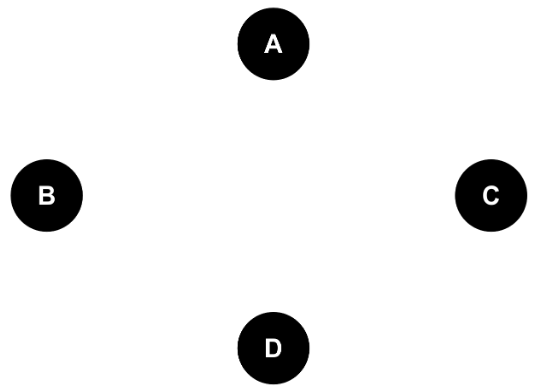
\includegraphics[width=0.4\textwidth]{TCC/imagens/grafos/turmas-vertices1.png}
     \caption{Turmas modeladas como um Grafo}
     \label{grafo-turmas1}
\end{figure}

Foi definido em nossa modelagem que uma aresta representaria a interseção de alunos entre duas turmas. Com isso toda turma que possuir alunos em comum irá receber uma aresta ($e$) que interligue os vértices ($v$ e $w$) referentes as respectivas turmas.

Observando novamente a tabela \ref{tabela-lista-turmas}, ao compararmos os alunos inscritos nas turmas A e B, notaremos que existem alguns alunos que pertencem a ambas turmas, como os alunos \textit{003, 006 e 009}.

Essa interseção observada irá gerar uma aresta no grafo que interliga os vértices \textbf{A} e \textbf{B}, como pode ser visto na figura \ref{grafo-turmas2}. Representando assim que ambas turmas possuem alunos em comum.

\begin{figure}[H]
     \centering
     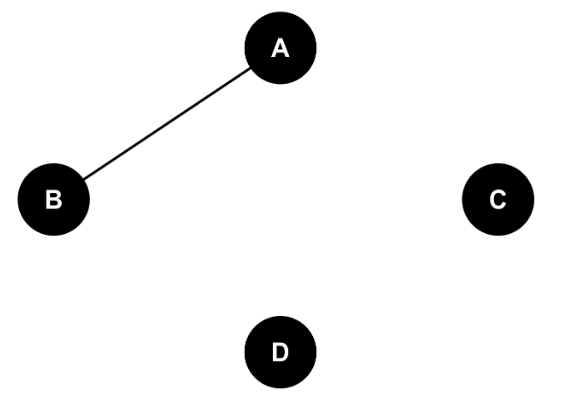
\includegraphics[width=0.4\textwidth]{TCC/imagens/grafos/turmas-vertices2.png}
     \caption{Representação do Grafo após comparar as turmas A e B}
     \label{grafo-turmas2}
\end{figure}

Repetindo o processo de observar a existência de alunos em comum entre cada par de turmas, iremos formar respectivamente os grafos exibidos nas figuras \ref{grafo-turmas3}, \ref{grafo-turmas4} e \ref{grafo-turmas5}.

\begin{figure}[H]
     \centering
     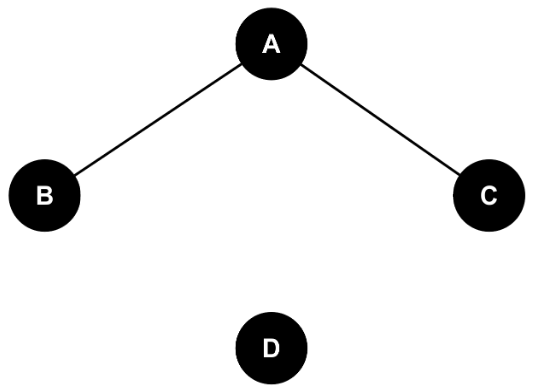
\includegraphics[width=0.4\textwidth]{TCC/imagens/grafos/turmas-vertices3.png}
     \caption{Representação do Grafo após comparar as turmas A e C}
     \label{grafo-turmas3}
\end{figure}

\begin{figure}[H]
     \centering
     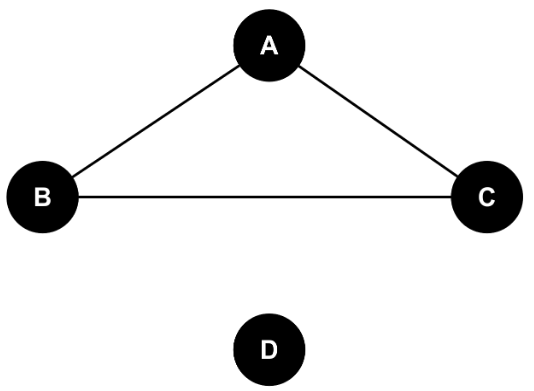
\includegraphics[width=0.4\textwidth]{TCC/imagens/grafos/turmas-vertices4.png}
     \caption{Representação do Grafo após comparar as turmas B e C}
     \label{grafo-turmas4}
\end{figure}

\begin{figure}[H]
     \centering
     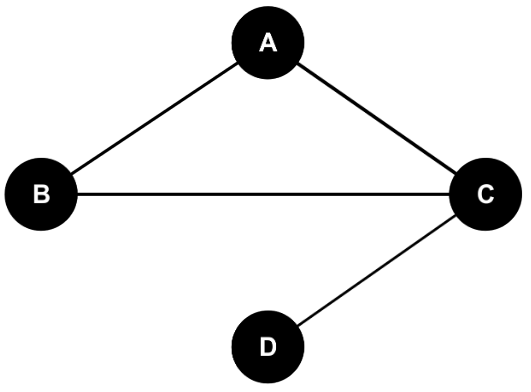
\includegraphics[width=0.4\textwidth]{TCC/imagens/grafos/turmas-vertices5.png}
     \caption{Representação do Grafo após comparar as turmas C e D}
     \label{grafo-turmas5}
\end{figure}

Finalizando o processo de identificação de interseções entre as turmas teremos o grafo de interseção das turmas da instituição, e através dele (figura \ref{grafo-turmas5}), podemos observar todas as turmas que possuem alunos em comum.

Agora que sabemos como transformar um conjunto de turmas em um grafo, precisaremos encontrar um meio de utilizar essa estrutura para simplificar a forma como criaríamos a grade de exames universitários.

A forma pela qual criaremos as grades de horários, será apresentada no capítulo de \ref{cap:solucao}, onde será utilizado o grafo criado no exemplo desse subcapítulo (figura \ref{grafo-turmas5}) para demonstrar os benefícios e limitações provenientes dessa modelagem e suas devidas soluções.





%%
%%
%%
%%


\chapter{Método de Solução}
\pagestyle{simple}
\label{cap:solucao}

Após realizar a modelagem na forma de um problema de grafo, iremos utilizar essa estrutura para criar uma grade de horário de provas que satisfaça as restrições do problema.

Considerando um grafo $G$ qualquer, definimos como as turmas pertencentes á $G$ como $V(G) = \{v_1, v_2, v_3, …, v_n\}$, ou seja, o conjunto de vértices $V(G)$ corresponderá às disciplinas ofertadas na instituição, sendo $n$ a quantidade de vértices do grafo $|V(G)|$ e de disciplinas ofertadas.

Definimos que os horários serão representados por números inteiros positivos $K = \{1, 2, 3, …, k\} \in \mathbf{N}$, sendo $k$ o número correspondente a quantidade máxima de horários para realização das provas.

Ao atribuirmos uma turma a um horário de prova, estaremos relacionando um elemento de $K$ á um vértice $v$ de $V(G)$.

Sendo $V(G) = \{v_1, v_2, v_3, v_4\}$ e $K = \{1, 2, 3, 4\}$, podemos realizar uma atribuição que gere o resultado apresentado na tabela a seguir:

\begin{table}[H]
    \centering
    \vspace{0.5cm}
    \renewcommand\arraystretch{1.5}
    \begin{tabular}{c|c}
     
        \textbf{Vértices ($V(G)$)} & \textbf{Horários ($K$)} \\ % Note a separação de col. e a quebra de linhas
        \hline                               % para uma linha horizontal
        	$v_1$ & 1 \\
$v_2$ & 2 \\
$v_3$ & 3 \\
$v_4$ & 4      % não é preciso quebrar a última linha
        \\
        \hline
    \end{tabular}
    \caption{Relação entre os vértices e os horários}
    \label{tabela-relacao1}
\end{table}




Dessa forma, teremos cada turma realizando a prova em um horário distinto. Como apresentado no capítulo \ref{cap:problema}, esse seria um exemplo de solução trivial para o problema.

Contudo, assim como explicado anteriormente, a solução trivial não é o foco do trabalho, dessa forma para se realizar a atribuição de turmas aos horários deveremos por uma ou mais turmas em um mesmo horário. 

Para definir quais provas poderão ser aplicadas em um mesmo horário, iremos considerar os alunos pertencentes á ambas turmas. Com isso, caso duas turmas não possuam alunos em comum, elas poderão realizar seus exames em um mesmo horário.

Para sabermos se as turmas possuem alunos em comum, realizamos a modelagem das turmas na forma de um grafo (conforme apresentado no capítulo \ref{cap:modelagem}), dessa maneira podemos visualizar a existência de relações de acordo com as arestas do grafo.

Agora, para realizarmos a atribuição das turmas em horários aproveitaremos a forma gráfica do grafo, atribuindo uma cor a cada horário.

Para demonstrar, iremos utilizar o grafo resultante da modelagem no capítulo \ref{cap:modelagem} (figura \ref{grafo-turmas5}), que utilizou como base os alunos e as turmas descritas na tabela \ref{tabela-lista-turmas}.

Caso tivéssemos quatro ou mais horários disponíveis, bastaria realizar a solução trivial para o problema, então definiremos que será necessário aplicar as provas dessas turmas em apenas três horários. Sendo assim, teremos $k = 3$ horários e $n = 4$ turmas.

Para facilitar a visualização das operações que serão realizadas, relacionaremos os horários que temos disponíveis para realização de prova á cores únicas, conforme a tabela abaixo:

\begin{table}[H]
    \centering
    \vspace{0.5cm}
    \renewcommand\arraystretch{1.5}
    \begin{tabular}{c|c}
     
        \textbf{Horário} & \textbf{Cor} \\ % Note a separação de col. e a quebra de linhas
        \hline                               % para uma linha horizontal
        	1 & Vermelho \\
2  & Azul \\
3 & Verde
        \\
        \hline
    \end{tabular}
    \caption{Relação entre horários e cores}
    \label{tabela-relacao2}
\end{table}


A partir disso iremos atribuir á primeira turma o primeiro horário, dessa forma podemos pintar o vértice \textbf{A} (correspondente a turma A) de vermelho (cor que corresponde ao horário 1), assim como pode ser observado na figura \ref{grafo-colorido1}.

\begin{figure}[H]
     \centering
     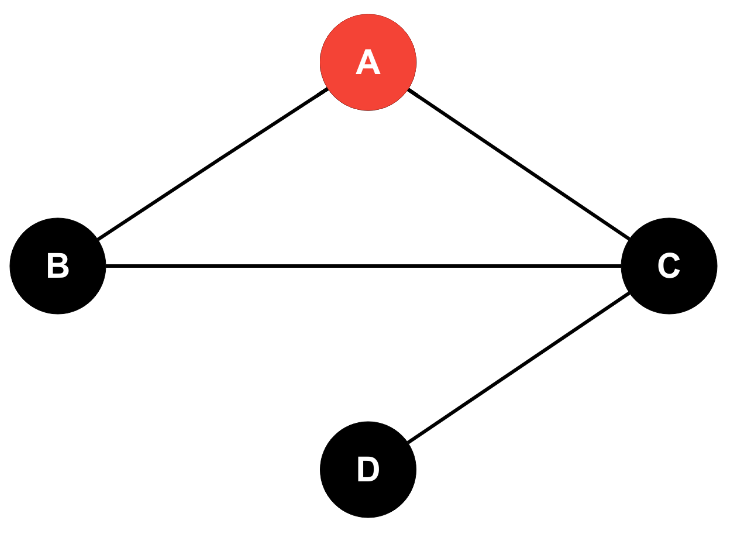
\includegraphics[width=0.4\textwidth]{TCC/imagens/grafos/colorindo1.png}
     \caption{Grafo após definir horário para turma A}
     \label{grafo-colorido1}
\end{figure}


Ao olhar para o vértice \textbf{B}, percebemos que a turma que ele representa possui alunos em comum com a turma representada pelo vértice \textbf{A}, logo, caso ambas as turmas necessitem fazer prova em um mesmo horário, esses alunos em comum terão que obrigatoriamente realizar a segunda chamada de uma das disciplinas.


Assim, visando evitar esse conflito de horários iremos atribuir a “turma B ”ao horário 2, com isso pintaremos o vértice \textbf{B} de Azul.

\begin{figure}[H]
     \centering
     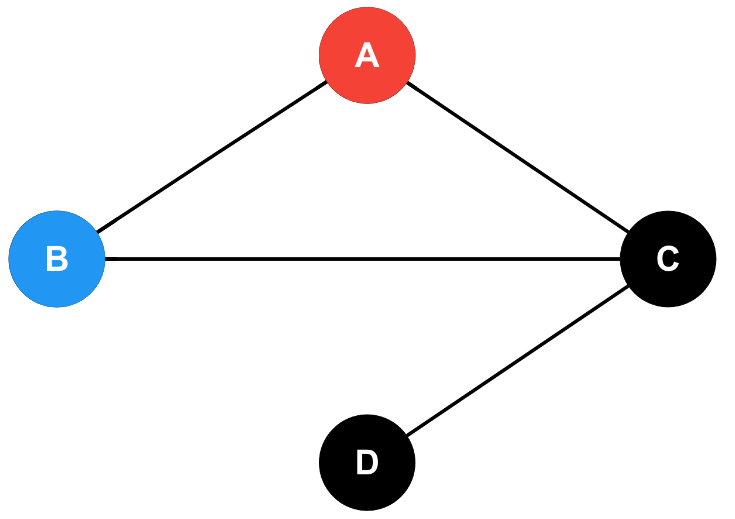
\includegraphics[width=0.4\textwidth]{TCC/imagens/grafos/colorindo2.png}
     \caption{Grafo após definir horário para turma B}
     \label{grafo-colorido2}
\end{figure}


Observando que o vértice \textbf{C} é adjacente (ligado por arestas)
 aos vértices \textbf{A} e \textbf{B}, sabemos que ele possui alunos em comum com ambas as turmas, dessa forma ele não deverá ser colocado em um horário diferente, assim atribuiremos ele ao horário 3 e pintaremos ele de verde.

\begin{figure}[H]
     \centering
     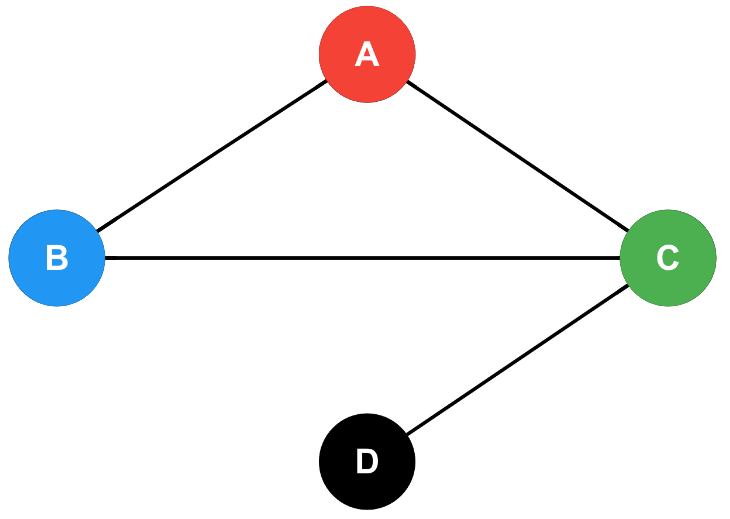
\includegraphics[width=0.4\textwidth]{TCC/imagens/grafos/colorindo3.png}
     \caption{Grafo após definir horário para turma C}
     \label{grafo-colorido3}
\end{figure}


O vértice \textbf{D}, é adjacente apenas ao vértice \textbf{C}, logo poderíamos pinta-lo de vermelho ou de azul, e dessa forma seus alunos realizariam a prova sem conflitos. Iremos então atribuí-lo ao horário 1 no mesmo horário que a turma A, e pintaremos o vértice D de vermelho.

Dessa forma podemos observar na figura \ref{grafo-colorido4} a distribuição das turmas em seus respectivos horários através do grafo com todos os seus vértices pintados.

\begin{figure}[H]
     \centering
     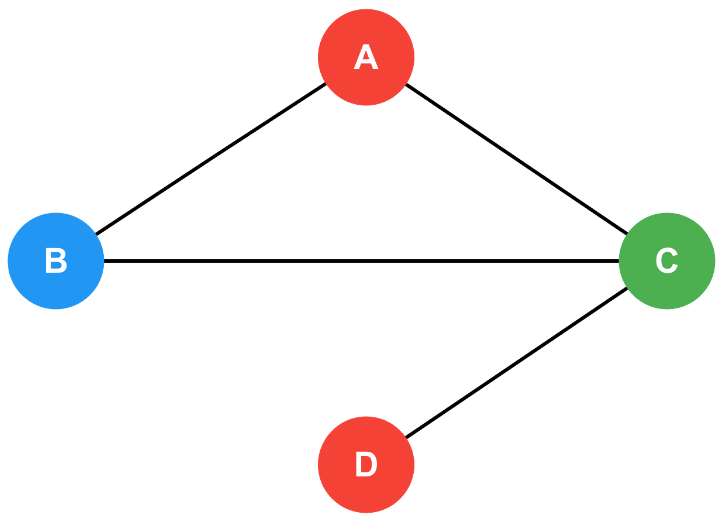
\includegraphics[width=0.4\textwidth]{TCC/imagens/grafos/colorindo4.png}
     \caption{Grafo após definir horário para turma D}
     \label{grafo-colorido4}
\end{figure}

Com isso obtemos como resultado, a grade de horários representada pela tabela a seguir:

\begin{table}[H]
    \centering
    \vspace{0.5cm}
    \renewcommand\arraystretch{1.5}
    \begin{tabular}{c|c}
     
        \textbf{Turmas} & \textbf{Horário} \\ % Note a separação de col. e a quebra de linhas
        \hline                               % para uma linha horizontal
        	A, D & 1 \\
B  & 2 \\
C & 3
        \\
        \hline
    \end{tabular}
    \caption{Alocação das turmas em três horários}
    \label{tabela-relacao3}
\end{table}



O processo de pintar os vértices do grafo, de forma que vértices adjacentes não recebam mesma cor, consiste em uma área muito estudada dentro da Teoria de Grafos, que é a Coloração de Grafos.

No caso específico apresentado, pode ser observado que realizar a alocação das turmas em horários, corresponde á busca por uma coloração própria de vértices do grafo.


\section{Coloração Própria de Vértices de um Grafo}


% [DEFINIÇÃO]

% O que é coloração

A coloração de um grafo qualquer é dada através da atribuição de rótulos aos elementos pertencentes ao grafo (vértices ou arestas), relacionamos esses rótulos à cores de forma a facilitar a visualização da coloração. Contudo para uma coloração ser válida ela precisa cumprir determinada restrição, elementos adjacentes (ou incidentes) não podem possuir mesma “cor”.

% Coloração de vértices

Entre os tipos de coloração existem as de vértices, arestas e total, que visam colorir tanto vértices quanto arestas. Para \citeonline{goldbarg_12} colorir os vértices de um grafo propriamente corresponde a atribuir cores aos vértices de forma que os vértices adjacentes recebam cores distintas.


\begin{figure}[H]
     \centering
     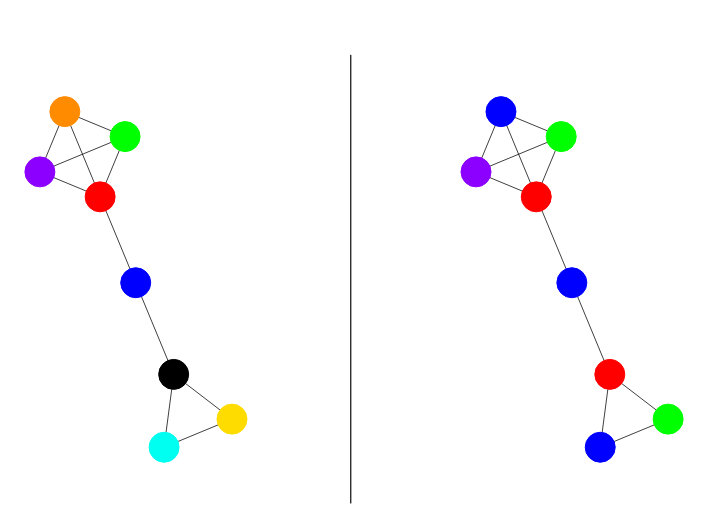
\includegraphics[width=0.4\textwidth]{TCC/imagens/grafos/grafo-propriamente.png}
     \caption{Grafo colorido propriamente}
     \label{grafo-propriamente}
\end{figure}


Uma coloração própria para os vértices de um grafo pode ser realizada ao se colorir cada vértice de uma cor diferente, dessa forma nenhum vértice adjacente (ou vizinho) terá mesma cor. No entanto quando pretendemos colorir os vértices buscando utilizar um número mínimo de cores, nos deparamos com um problema que pode não ser muito simples de se resolver.

% Número Cromático
\begin{definition} 
O menor número possível de cores para se colorir um grafo é chamado de \textbf{número cromático do grafo} denotado por $\chi(G)$. 
\end{definition}

% Coloração própria
Encontrar uma coloração com o número cromático do grafo é classificado como um problema NP-Completo quando $\chi(G) \geq 3$ . Dessa forma, encontrar tal coloração é classificado como um dos problemas mais difíceis estudados na computação.


% [ORIGEM]

Sendo uma das áreas mais estudadas na matemática e computação atualmente, a coloração de grafos se popularizou através da demonstração para uma conjectura existente por mais de um século. O matemático Francis Guthrie conjecturou em 1852 que \textbf{quatro cores eram o suficiente para se colorir um mapa}. Por se tratar de um problema muito difícil a demonstração matemática foi apresentada apenas em 1960 com auxílio do poder computacional \cite{lima_14}.

\begin{figure}[H]
     \centering
     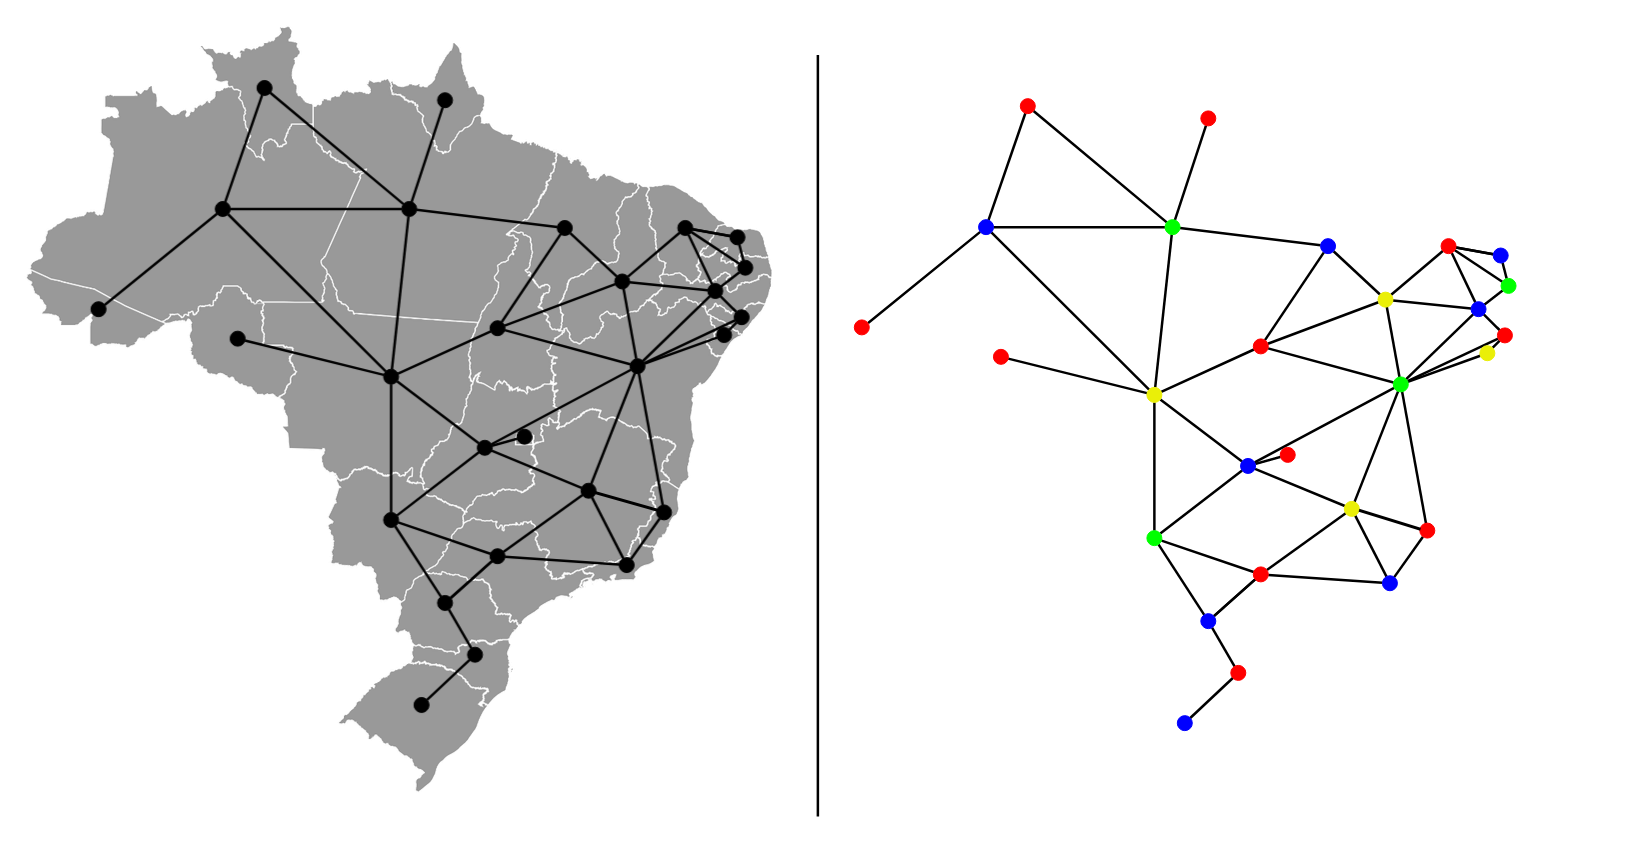
\includegraphics[width=0.8\textwidth]{TCC/imagens/grafos/grafo-mapa4cores.png}
     \caption{Exemplo de 4-coloração do mapa do Brasil}
     \label{grafo-mapa4cores}
\end{figure}

Para essa demonstração foi utilizada uma estrutura de grafo, onde buscava-se modelar um mapa de forma que os vértices representassem locais e esses vértices possuiriam arestas caso possuíssem fronteira. Então ao se colorir propriamente o grafo era possível demonstrar que a mesma coloração poderia ser realizada no mapa, afim de que países que tenham fronteiras em comum não possuam mesma cor.


% [APLICAÇÕES]

Desde então muitos outros modelos e aplicações utilizaram da coloração de grafos como uma forma de solução para um problema abstrato ou concreto.

Além da clássica aplicação concreta da coloração de grafos para se colorir mapas, existem ainda muitas outras formas de se utilizar essa ferramenta matemática.

Algumas aplicações em que se é utilizado a coloração de grafos, e que são formalmente apresentadas em diversos trabalhos e pesquisas acadêmicas, estão formas de se resolver jogos como \textit{SUDOKU}, realização de transporte de componentes que podem ou não se misturados, visando minimizar custos e aumentar a segurança, armazenamento seguro ou inteligente de itens conforme suas características, visando deixa-los mais próximos ou distantes entre muitos outros observados na literatura. 

% [ALGORITMOS]

Existem diversas propostas de algoritmos para encontrar uma coloração própria de um grafo, alguns se destacam por sua simplicidade e desempenho. Desde métodos exatos até heurísticas, as propostas de solução para o problema das colorações são as mais diversificadas possíveis e em alguns casos, a utilização dessas soluções não é o suficiente para se encontrar uma coloração que atenda as condições do problema modelado.

Nesse caso busca-se identificar os fatores que contribuem para a não obtenção do resultado ideal, e assim modelar o problema novamente solucionando então esses possíveis empecilhos.

\section{Limitação no número de Horários de Prova}

A solução do problema de exames universitários por meio da coloração própria de vértices, não resolverá todos os casos possíveis, já que é possível existir um caso onde a quantidade de horários disponíveis para realização da prova $k$ é menor que o número cromático do grafo $\chi(G)$.

\begin{figure}[H]
     \centering
     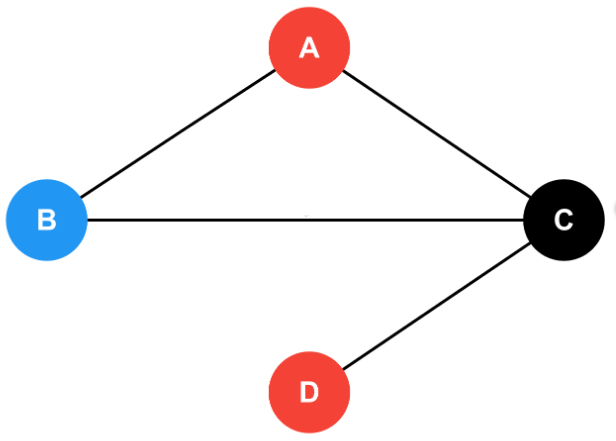
\includegraphics[width=0.4\textwidth]{TCC/imagens/grafos/grafo-colorido-2k.png}
     \caption{Qual cor devo atribuir ao vértice C?}
     \label{grafo-k2}
\end{figure}



Nesse caso, como uma coloração própria não será suficiente, adotaremos uma nova forma de solução. 

Considerando que não será possível separar todas as turmas que possuem alunos em comum em horários de forma que não gere conflitos, iremos buscar uma solução que minimize a quantidade de provas de segunda chamada, ou seja, a número de alunos prejudicados.

Para sabermos quantos alunos estarão sendo prejudicados precisaremos incluir mais uma etapa em nossa modelagem.

Iremos atribuir às arestas do grafo um peso, correspondente a quantidade de alunos que pertencem às duas turmas. Dessa forma teremos um Grafo Ponderado em Arestas.



\section{Grafos Ponderados em Arestas}

Retornando a tabela \ref{tabela-lista-turmas} no capítulo \ref{cap:modelagem}, observamos agora não apenas a existência de alunos em comum às turmas, mas também a quantidade de alunos.

Ao realizar esse processo e escrevermos sobre as arestas a quantidade de alunos na interseção, teremos um grafo ponderado como na figura \ref{grafo-ponderado1}.

\begin{figure}[H]
     \centering
     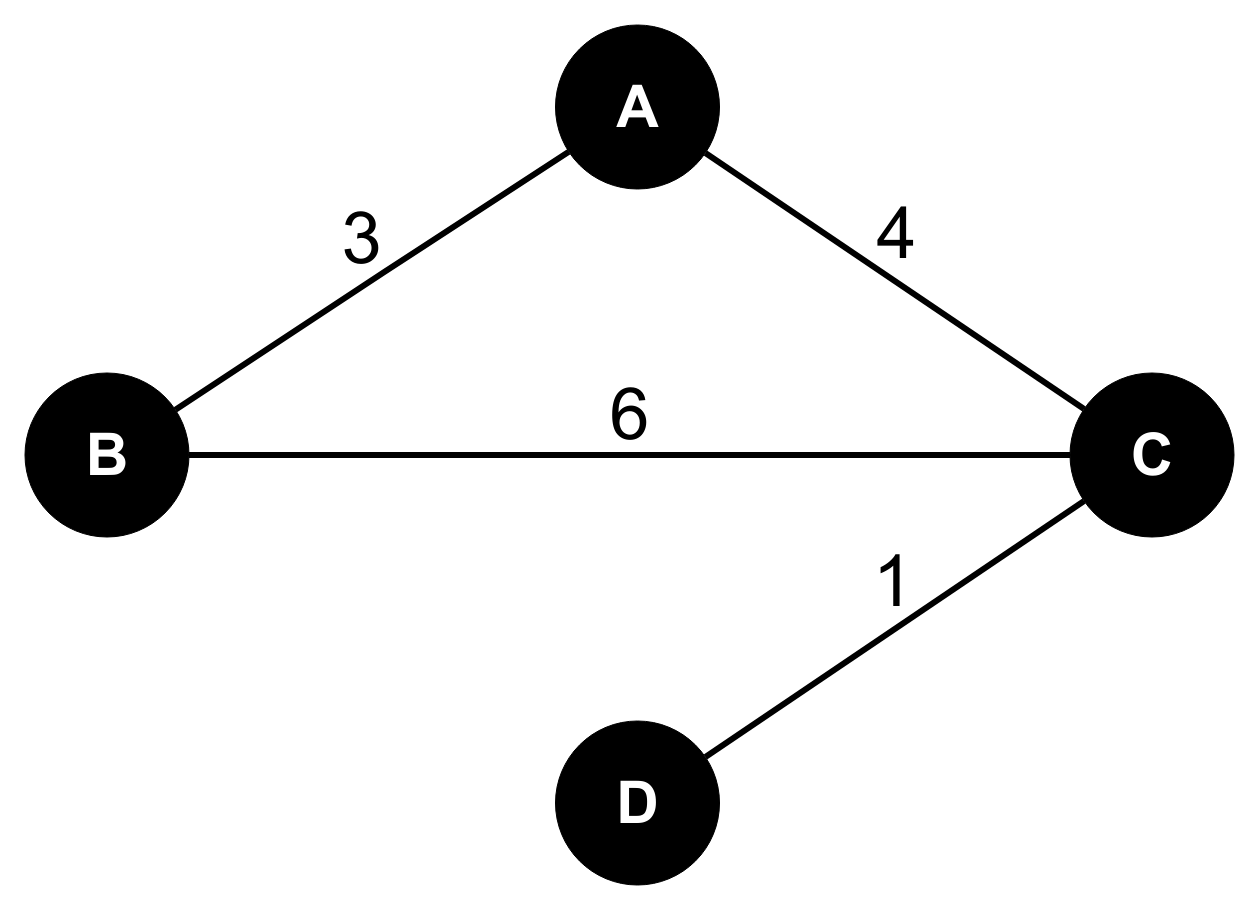
\includegraphics[width=0.4\textwidth]{TCC/imagens/grafos/grafo-ponderado.png}
     \caption{Grafo ponderado em arestas}
     \label{grafo-ponderado1}
\end{figure}


Utilizando do grafo ponderado conseguimos observar quantos alunos seriam prejudicados caso alocarmos quaisquer duas turmas em um mesmo horário. 

Colorir o grafo agora consistirá em encontrar uma coloração não própria cuja soma dos pesos das arestas incidentes em vértices coloridos com mesma cor seja o menor possível.  

Esse processo é chamado de {Generalized Graph Coloring}, onde efetuamos um tipo especial de coloração de modo a atingir algum objetivo pré-estabelecido.




\section{Generalized Graph Coloring Problem}

\begin{definition} 
 \citeonline{vredeveld_02}, define o $k$-GGCP como sendo um problema que consiste em um grafo $G(V, E)$, uma função de peso $z:E \rightarrow  Z$ sobre as arestas, e um número inteiro $k \geq 2$.

Onde deseja-se encontrar uma atribuição de cores $c:V \rightarrow  \{1, ..., k\}$ dos vértices que minimize o peso total das arestas monocromáticas do grafo, isto é, arestas que incidem em vértices com mesma cor.

\end{definition}

Usando o exemplo da figura \ref{grafo-k2}, onde não sabemos como colorir o vértice \textbf{C}, pela ausência de uma terceira cor, iremos testar como seria se escolhermos uma das duas cores para colorir esse vértice.

\begin{figure}[H]
     \centering
     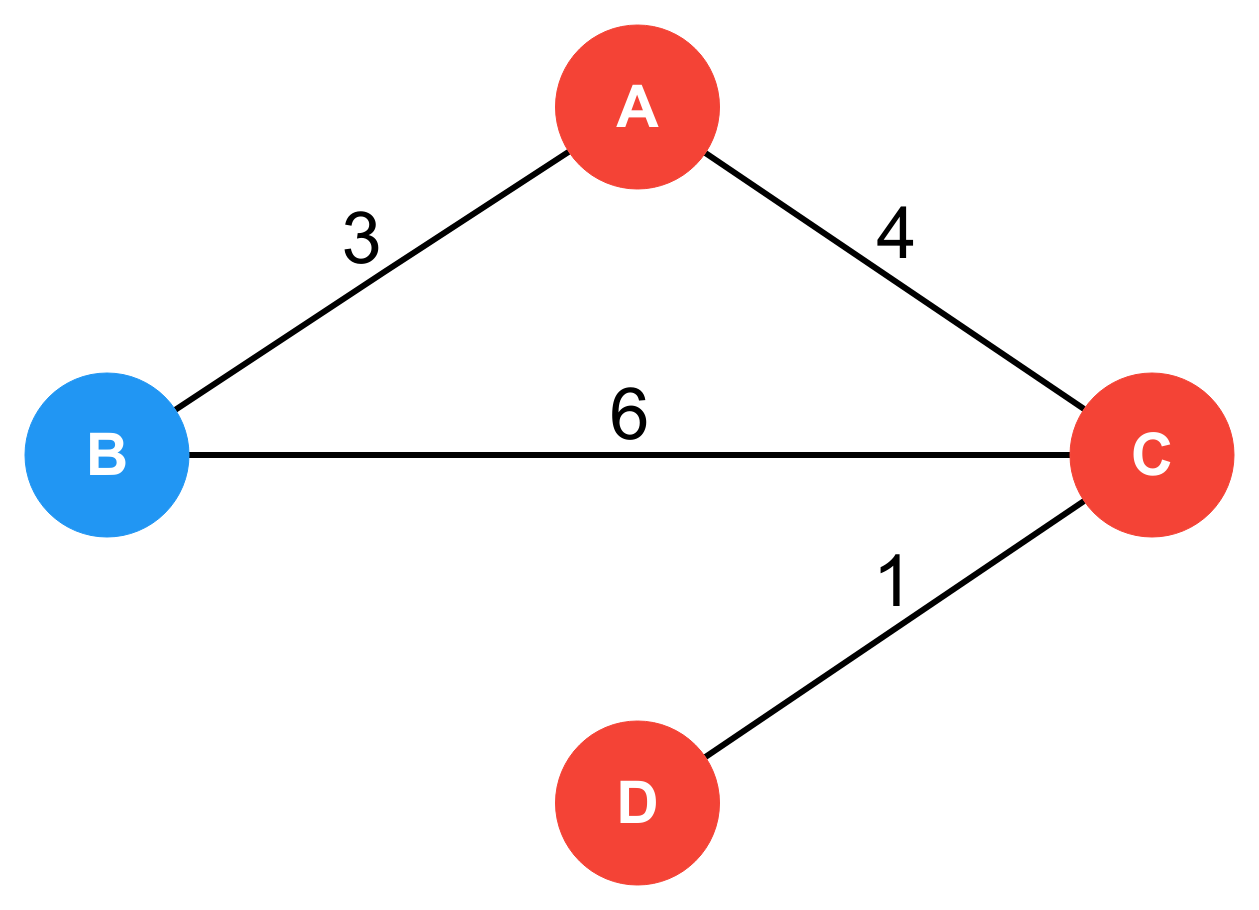
\includegraphics[width=0.4\textwidth]{TCC/imagens/grafos/grafo-ponderado-colorido.png}
     \caption{Caso 1: Grafo colorido com vértice C vermelho}
     \label{grafo-ponderado-colorido1}
\end{figure}


Caso optemos por colorir o vértice \textbf{C} de vermelho, teremos as turmas A, C e D em um mesmo horário de prova. Ao somar o peso das arestas que incidem nesses vértices, temos que cinco provas de segunda chamada serão necessárias, sendo quatro alunos prejudicados nas turmas A e C, e um aluno nas turmas C e D.

\begin{figure}[H]
     \centering
     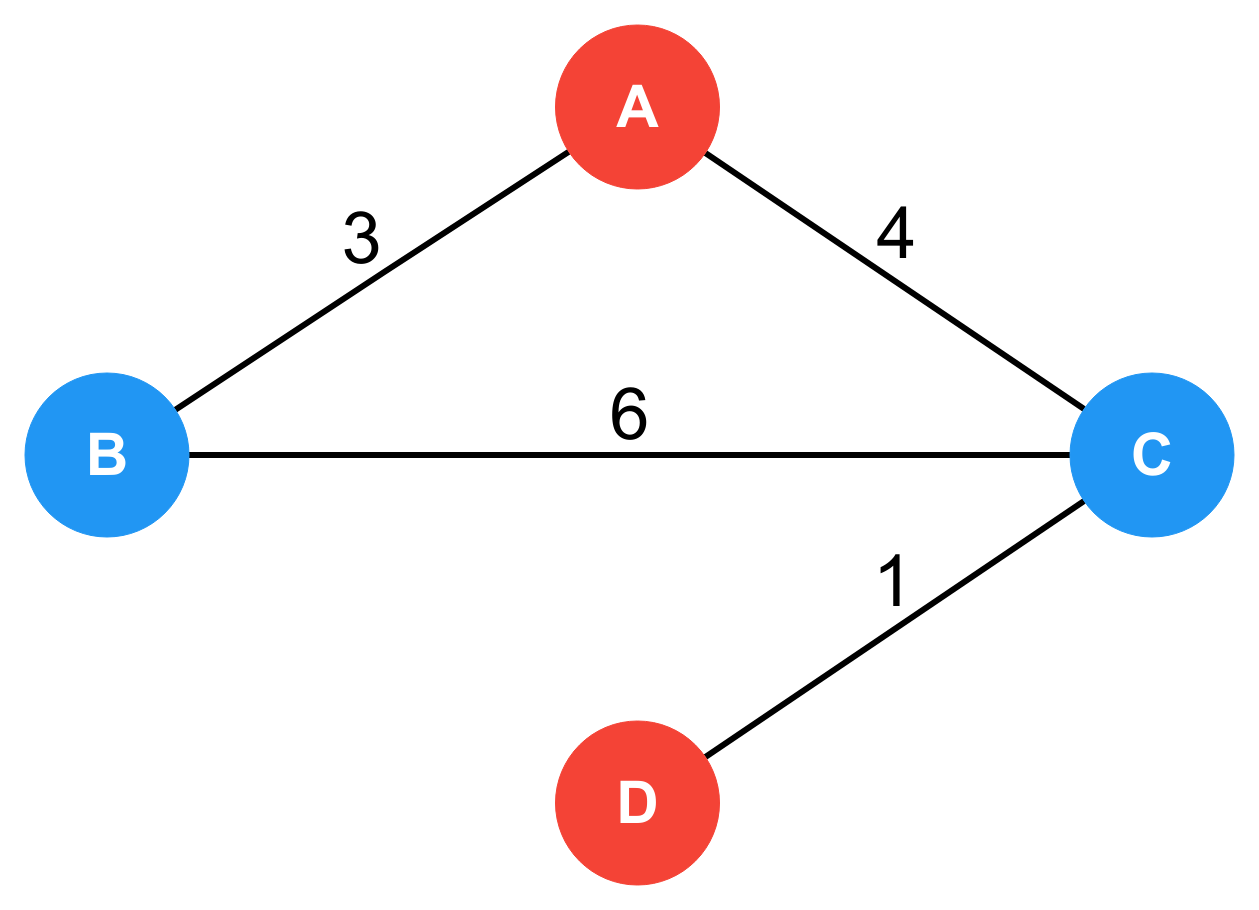
\includegraphics[width=0.4\textwidth]{TCC/imagens/grafos/grafo-ponderado-colorido-v2.png}
     \caption{Caso 2: Grafo colorido com vértice C azul}
     \label{grafo-ponderado-colorido2}
\end{figure}


Escolhendo colorir o vértice de azul, temos a “turma C ”no mesmo horário que a “turma B', o que causaria conflito para os seis alunos que pertencem às duas turmas.

Ao buscar a distribuição que cause o menor número de conflitos chegaremos à coloração representada na figura \ref{grafo-ponderado-colorido3}, no qual podemos observar que teremos apenas os três alunos que fazem parte das turmas A e B prejudicados.

\begin{figure}[H]
     \centering
     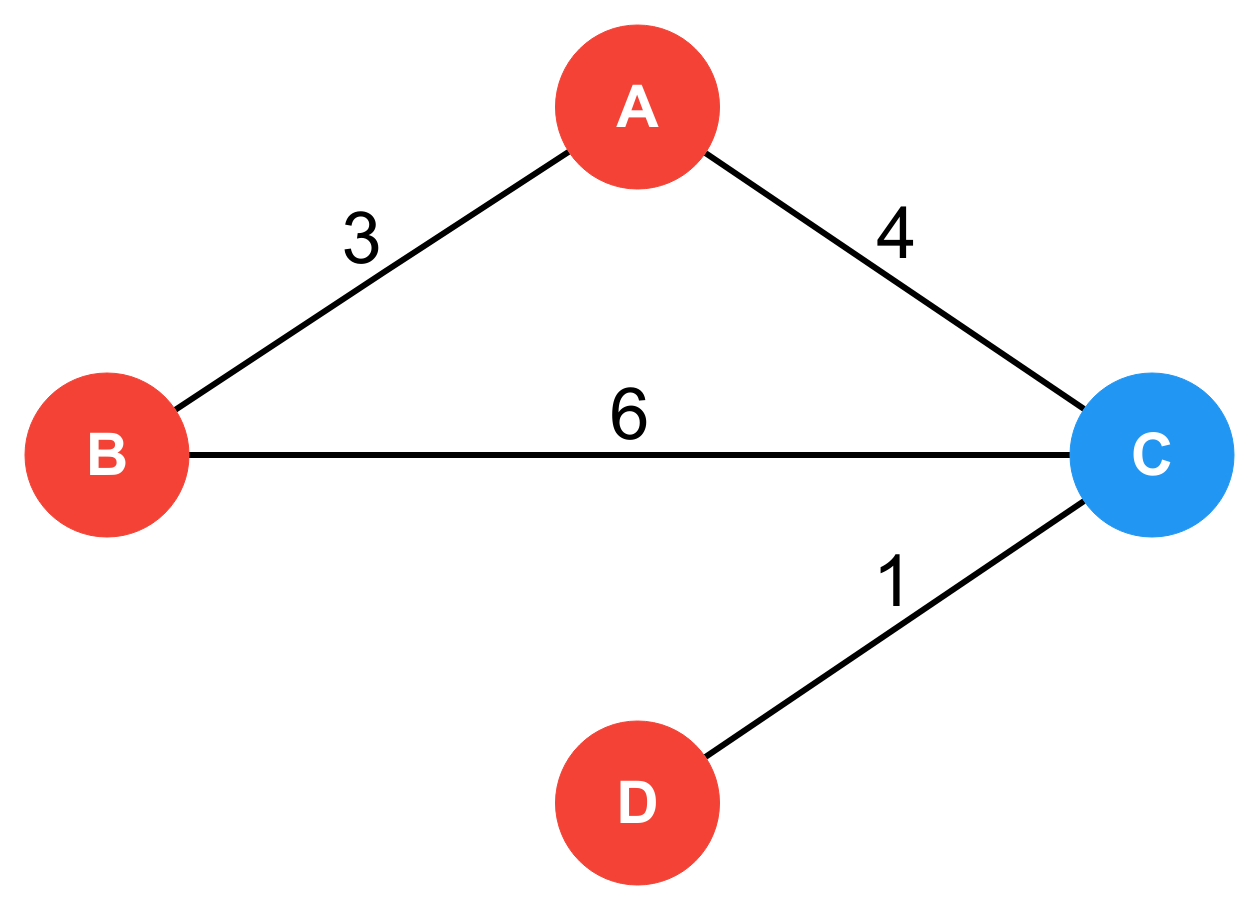
\includegraphics[width=0.4\textwidth]{TCC/imagens/grafos/grafo-ponderado-colorido-v3.png}
     \caption{Melhor coloração com duas cores para o Grafo}
     \label{grafo-ponderado-colorido3}
\end{figure}


Dessa forma o resultado para a grade de horário de prova para as turmas do exemplo será:

\begin{table}[H]
    \centering
    \vspace{0.5cm}
    \renewcommand\arraystretch{1.5}
    \begin{tabular}{c|c}
     
        \textbf{Turma} & \textbf{Horário} \\ % Note a separação de col. e a quebra de linhas
        \hline                               % para uma linha horizontal
        	A, B, C & 1 \\
C  & 2
        \\
        \hline
    \end{tabular}
    \caption{Relação entre horários e cores}
    \label{tabela-relacao4}
\end{table}



Causando dessa forma \textbf{três provas de segunda chamada} por consequência da alocação.



\section{Complexidade do Problema e Viabilidade de Solução}

O PPHC é um problema classificado NP-Completo por \citeonline{garey79}, para todo $k \geq 3$, isso é, para qualquer quantidade de horários maior ou igual a $3$ quando $k$ não for fixo, \citeonline{vredeveld_02} define o problema como NP-Difícil quando o valor $k$ é fixo, por ser equivalente ao MaxCut quando $k = 2$ e equivalente ao problema Max $k$-Cut para qualquer $k \geq 3$, enquanto estes são classificados como NP-Difícil.  

% O problema foi resolvido utilizado o método de força bruta, onde se busca exaustivamente por todas as situações possível a fim de encontrar a melhor solução (cite).

% [O que é NP-Completude e NP-Completo]


Na teoria da computação a complexidade de um problema está diretamente atrelada a capacidade que temos de soluciona-la computacionalmente e o tempo que custará para isso. A maioria dos problemas podem ser divididos em duas diferentes classes P e NP. 

São considerados P os problemas que possuem pelo menos um algoritmo capaz de resolve-lo em tempo polinomial, já um problema NP é um problema não determinístico, porém que pode ter uma solução verificada em tempo polinomial.

% (Pegar definição resumida de problema NP-Completo)
Um subconjunto dos NP é chamado de NP-Completo, sendo uma classe de problemas em que para se pertencer a ela, o problema deve ser classificado como NP e deve ser possível equipara-lo a outro problema já classificado como NP-Completo, ou seja, por definição os NP-Completos são uma classe que ao se encontrar uma solução para um dos problemas os demais também serão solucionados devido a suas semelhanças.

% [O que é um problema NP-Difícil]
Outro subconjunto dos NP são os NP-Difíceis, que são classificados como problemas pelo menos tão difíceis quanto os NP-Completos.


% [O que um problema NP-Difícil interfere na solução]

Ao se deparar com situações desse tipo, o mais comum na literatura é buscar soluções não exatas. Assim, muitos trabalhos publicados para problemas similares ao apresentado aqui, demonstraram bons resultados utilizando diversas técnicas não exatas para se encontrar uma solução, com uso de heurísticas e meta-heurísticas como: \textit{GRASP}, \textit{Busca Tabu}, \textit{Algoritmos Genéticos}, entre muitos outros \cite{rocha13}.

\section{Algoritmo Desenvolvido Inicialmente}
\label{sec-alg-desv}

Um algoritmo foi desenvolvido inicialmente, visando encontrar a melhor alocação de turmas em uma quantidade limitada de horários.

Esse algoritmo possui como entradas: 
\begin{itemize}
    \item[(A)] Um Grafo de interseção ponderado nas arestas $G$;
    \item[(B)] a quantidade $k$ de horários de prova disponíveis.
\end{itemize}
 

E como saída:
\begin{itemize}
    \item[(C)] A coloração $c$  (ou $c^{min}$) com menor custo obtido;
    \item[(D)] a quantidade $P_c$ de provas de segunda chamada necessárias com a coloração de menor custo. 
\end{itemize}
 

A entrada e a saída gerada pelo algoritmo consistia em arquivos de texto e o algoritmo apresentou bons resultados para uma série de testes que foram efetuados.

O método pelo qual o algoritmo buscava a melhor solução consistia em uma busca exaustiva por força bruta, na qual todas as combinações possíveis eram testadas e tinham seus resultados comparados, de modo a encontrar a solução com menor valor $p$ de provas de segunda chamada.

Apesar da garantia da obtenção de uma solução ótima para o problema, o custo computacional (e tempo de processamento) eram muito elevados para grandes instâncias com muitos horários de prova. Visando encontrar uma solução mais viável para grandes instâncias foi proposta a criação de uma heurística que nos permitisse encontrar uma solução boa com menor custo computacional.

\section{Heurística Proposta}


Para desenvolver a heurística foi utilizado como base o bem conhecido algoritmo chamado LF (\emph{Largest-first}), também chamado de método heurístico guloso de coloração própria de vértices de um grafo.

Esse algoritmo foi proposto inicialmente por \citeonline{welsh-powell67} e se baseia na estratégia de escolher colorir primeiramente os vértices que possuem maior grau, ordenando os vértices de acordo com o grau e os colorindo seguindo essa sequência.


\begin{figure}[H]
     \centering
     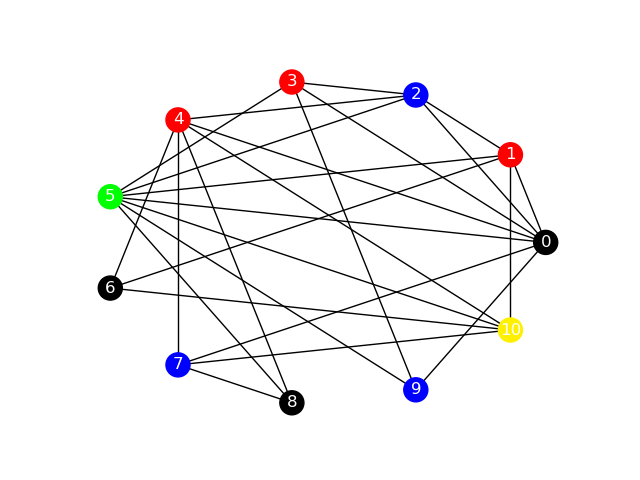
\includegraphics[width=0.7\textwidth]{TCC/imagens/grafos/20_11_50_10_6.png}
     \caption{Exemplo de Grafo colorido com algoritmo inicial }
     \label{grafo-20_11_50_10_6}
\end{figure}


\noindent\begin{minipage}{\linewidth}
\lstset{numbers=left, numberstyle=\tiny, stepnumber=1, numbersep=15pt}

\lstinputlisting[frame=tb,caption=Implementação do LF em Python,
  captionpos=b,belowcaptionskip=2cm, xleftmargin=5.0ex,
  label=zebra,language=python,label={alg-welsh-powell}]{arquivos/welsh-powell.py}
\end{minipage}

O algoritmo apresentado em \ref{alg-welsh-powell} foi desenvolvido inicialmente buscando encontrar colorações onde a quantidade de horários de provas disponíveis eram maiores ou iguais ao número cromático do grafo $\chi(G)$. Porém, conforme o problema evoluiu para um cenário onde deseja-se encontrar uma solução que satisfaça também modelos onde a quantidade de horários disponíveis seja menor que o número cromático do grafo, foi necessário uma mudança na estratégia.

Ao implementar o método por busca exaustiva citado na seção \ref{sec-alg-desv},  notou-se a necessidade de se obter uma solução em um menor tempo de processamento, ao se observar que em modelos com muitas turmas e muitos horários esse tempo de execução poderia dificultar ou até impossibilitar a utilização da mesma.

Foi então proposto um algoritmo adaptado do LF, observado a seguir, onde seria priorizada a coloração com diferentes cores dos vértices adjacentes as arestas de maior peso do grafo, ao invés do vértice de maior grau, como no algoritmo clássico de \citeonline{welsh-powell67}.

O algoritmo proposto pode ser exemplificado através dos passos apresentados através da tabela a seguir.


\begin{table}[H]
    \centering
    \vspace{0.5cm}
    \renewcommand\arraystretch{1.5}
    \begin{tabular}{c|l}
     
        \textbf{Passo} & \textbf{Ação} \\ % Note a separação de col. e a quebra de linhas
        \hline                               % para uma linha horizontal
        	1 & Buscar a aresta $vw$ com maior peso do Grafo, \\ & cujo o vértice $v$ ou $w$ não possuam cor. \\
            2  & Verificar se o vértice $v$ possui uma cor. \\
            3  & Selecionar uma cor $i$ para colorir o vértice $v$. \\
            4  & Verificar se o vértice $v$ pode ser colorido com a cor $i$. \\
            5  & Colorir o vértice $v$ com a cor $i$. \\
			6  & Verificar se o vértice $w$ possui uma cor. \\
            7  & Selecionar uma cor $j$ para colorir o vértice $w$. \\
            8  & Verificar se o vértice $w$ pode ser colorido com a cor $j$. \\
            9  & Colorir o vértice $w$ com a cor $j$. \\
            10 & Repetir o \textbf{passo 1} para a próxima aresta até que \\ & todos os vértices estejam coloridos.
        \\
        \hline
    \end{tabular}
    \caption{Passos para serem executados pela heurística}
    \label{tabela-heuristica}
\end{table}

A cada interação um novo par de vértices $uv$ são selecionados e duas cores são escolhidas para colori-los, contudo em caso de um resultado positivo o ao executar o passo 2 o algoritmo deverá pular para o passo 6. 

Caso não seja possível colorir um vértice com determinada cor, em função dele ser adjacente a outro vértice de mesma cor, o algoritmo deve retornar ao passo anterior e selecionar uma nova cor, se não houverem cores disponíveis o vértice será colorido om a cor que incide na aresta de menor peso.

A seguir está o código em linguagem C que tem como objetivo implementar os passos da heurística a fim de encontrar uma coloração ótima em um tempo reduzido de execução em comparação com o método de busca exaustiva.

\vspace{15pt}

\lstset{ numbers=left, numberstyle=\tiny, stepnumber=1, numbersep=15pt}

\lstinputlisting[frame=tb,caption=Heurística Proposta em C,
  captionpos=b,belowcaptionskip=2cm, xleftmargin=5.0ex,
  label=zebra,language=c,label={heuristica-proposta}]{arquivos/heuristica-proposta.c}

Após desenvolver um modelo no qual pudéssemos representar as turmas e as relações de interseção de alunos entre elas, buscamos então demonstrar um algoritmo capaz de solucionar os desafios apresentados ao longo do capítulo de forma a gerar uma programação de horários de prova com mínimos conflitos de horários de prova para os alunos e consequente aplicação de avaliações de segunda chamada.

Contudo, para possibilitar uma utilização mais diversificada da solução. Foi proposto um sistema, que será apresentado no capítulo \ref{cap:software}, no qual um usuário com menor conhecimento técnico fosse capaz de gerar grades de horários de prova.